% !TEX root = Document.tex
%!TeX spellcheck = fr
\Chapter{Inspection d'éoliennes par UAV}\label{sec:uav}

Dans ce chapitre nous abordons l'automatisation d'inspection d'éoliennes par un véhicule aérien autonome. Ce projet a été réalisé conjointement avec une compagnie privée opérant dans le secteur des drones commerciaux.
% la compagnie Microdrones Canada Inc.

\section{Description du problème et méthode d'inspection}

Les éoliennes doivent régulièrement être inspectées pour détecter et réparer le plus tôt possible les failles structurelles qui peuvent apparaître avec le temps à cause des intempéries ou quand elles sont frappées par la foudre. La peinture recouvrant celles-ci étant moins élastique que le composite de fibre de verre dont elles sont construites, un défaut structurel se manifeste inévitablement à la surface de la pale sous la forme de fissures ou de trous. Une inspection visuelle régulière peut donc être réalisée pour déceler et réparer toute irrégularité dans la structure avant qu'un bris catastrophique ne se produise.

En temps normal, une inspection se fait par une équipe de deux personnes devant grimper l'éolienne. L'équipe attend d'abord que le vent fasse tourner le rotor jusqu'à ce que la pale à examiner pointe vers le sol. À ce moment, le frein est enclenché et l'angle d'inclinaison des pales est ajusté pour que le vent ne crée pas de couple sur le rotor. L'équipe grimpe ensuite la tour jusqu'au sommet, ce qui peut prendre une dizaine de minutes si l'ascenseur est non fonctionnel, chose qui arrive fréquemment. Une fois rendu au rotor, un frein mécanique secondaire est activé pour bloquer la rotation des pales. L'équipe fait ensuite une descente en rappel le long de la pale pour faire l'inspection visuelle et tactile de la surface. Une fois l'inspection terminée le processus est recommencé pour les deux autres pales. Inspecter une éolienne peut prendre entre deux et quatre heures selon le nombre de bris à documenter.

%En plus de prendre beaucoup de temps, les inspection d'éoliennes posent un réel risque au niveau de la santé et sécurité des travailleurs nottament à cause des chutes possibles dans la tour pouvant faire plus d'une centaine de pieds de haut ou aussi par le fait de devoir naviguer des espaces confins pour se rendre au sommet de la tour \citep{Osha2017}. Ainsi, automatiser les inspections bénéfierait directement la santé des travailleurs et permetterait de sauver du temps et de l'argent.

Certains opérateurs d'UAV, offrent maintenant des services d'inspection d'éoliennes. Une caméra haute définition est montée sur un cardan stabilisateur à trois axes, lui-même monté sur le véhicule. Ce dernier est parfois aussi augmenté d'un télémètre permettant au pilote de savoir à quelle distance il est de la structure, chose difficile à estimer lorsque le véhicule est à 100 mètres d'altitude. Ces inspections peuvent prendre jusqu'à trois employés, dont un pilote, un opérateur pour la caméra et un observateur sous l'éolienne.

Le but du projet est d'explorer les solutions possibles pour réaliser un système capable de piloter un quadricoptère de façon autonome autour des pales d'une éolienne à l'aide de capteurs peu coûteux avec seulement un pilote de sécurité de présent et le moins d'informations \emph{a priori}. Ce projet peut aussi servir de tremplin vers un projet dans lequel aucun humain n'interviendrait, par exemple pour une flotte d'UAV chargée d'inspecter régulièrement un parc éolien entier. Puisque man\oe uvrer précisément autour des pales demanderait l'usage de capteurs dépassant le budget du projet et nécessiterait que l'UAV soit équipé de capteurs de position haute précision tel qu'un GPS différentiel, nous simplifions le problème en un problème à deux dimensions où le véhicule cherche à suivre le bord d'attaque (ou le bord de fuite) des pales. Deux approches ont été développées, l'une entièrement au moyen de scanners laser et l'autre par caméras stereo.

La mission se divise en deux phases: l'approche du rotor et le suivi de ses pales qui peuvent être gérées par une simple machine à états finis. Pour l'approche du rotor, nous comparons une approche à longue distance au moyen de traitement d'images à une approche à tâtons où l'UAV remonte la tour au moyen de scanners lasers. Pour le suivi des pales, nous comparons encore une méthode par traitement d'images à une méthode de suivie à tâtons. La compagnie pour laquelle nosu travaillons désirait que le système soit implémenté sur
%la compagnie Microdrones,
quadricoptère md4-1000. Nous installons sur le véhicule deux scanners lasers LeddarTech Vu8, l'un horizontal et l'autre vertical, ainsi qu'une caméra stéréo ZED. Il est à noter que ces capteurs ne servent qu'à la navigation de l'UAV alors que la caméra haute définition sur stabilisateur demeure le moyen par lequel prendre des photos des défauts à la surface des pales.

\begin{figure}[htp]
  \centering
  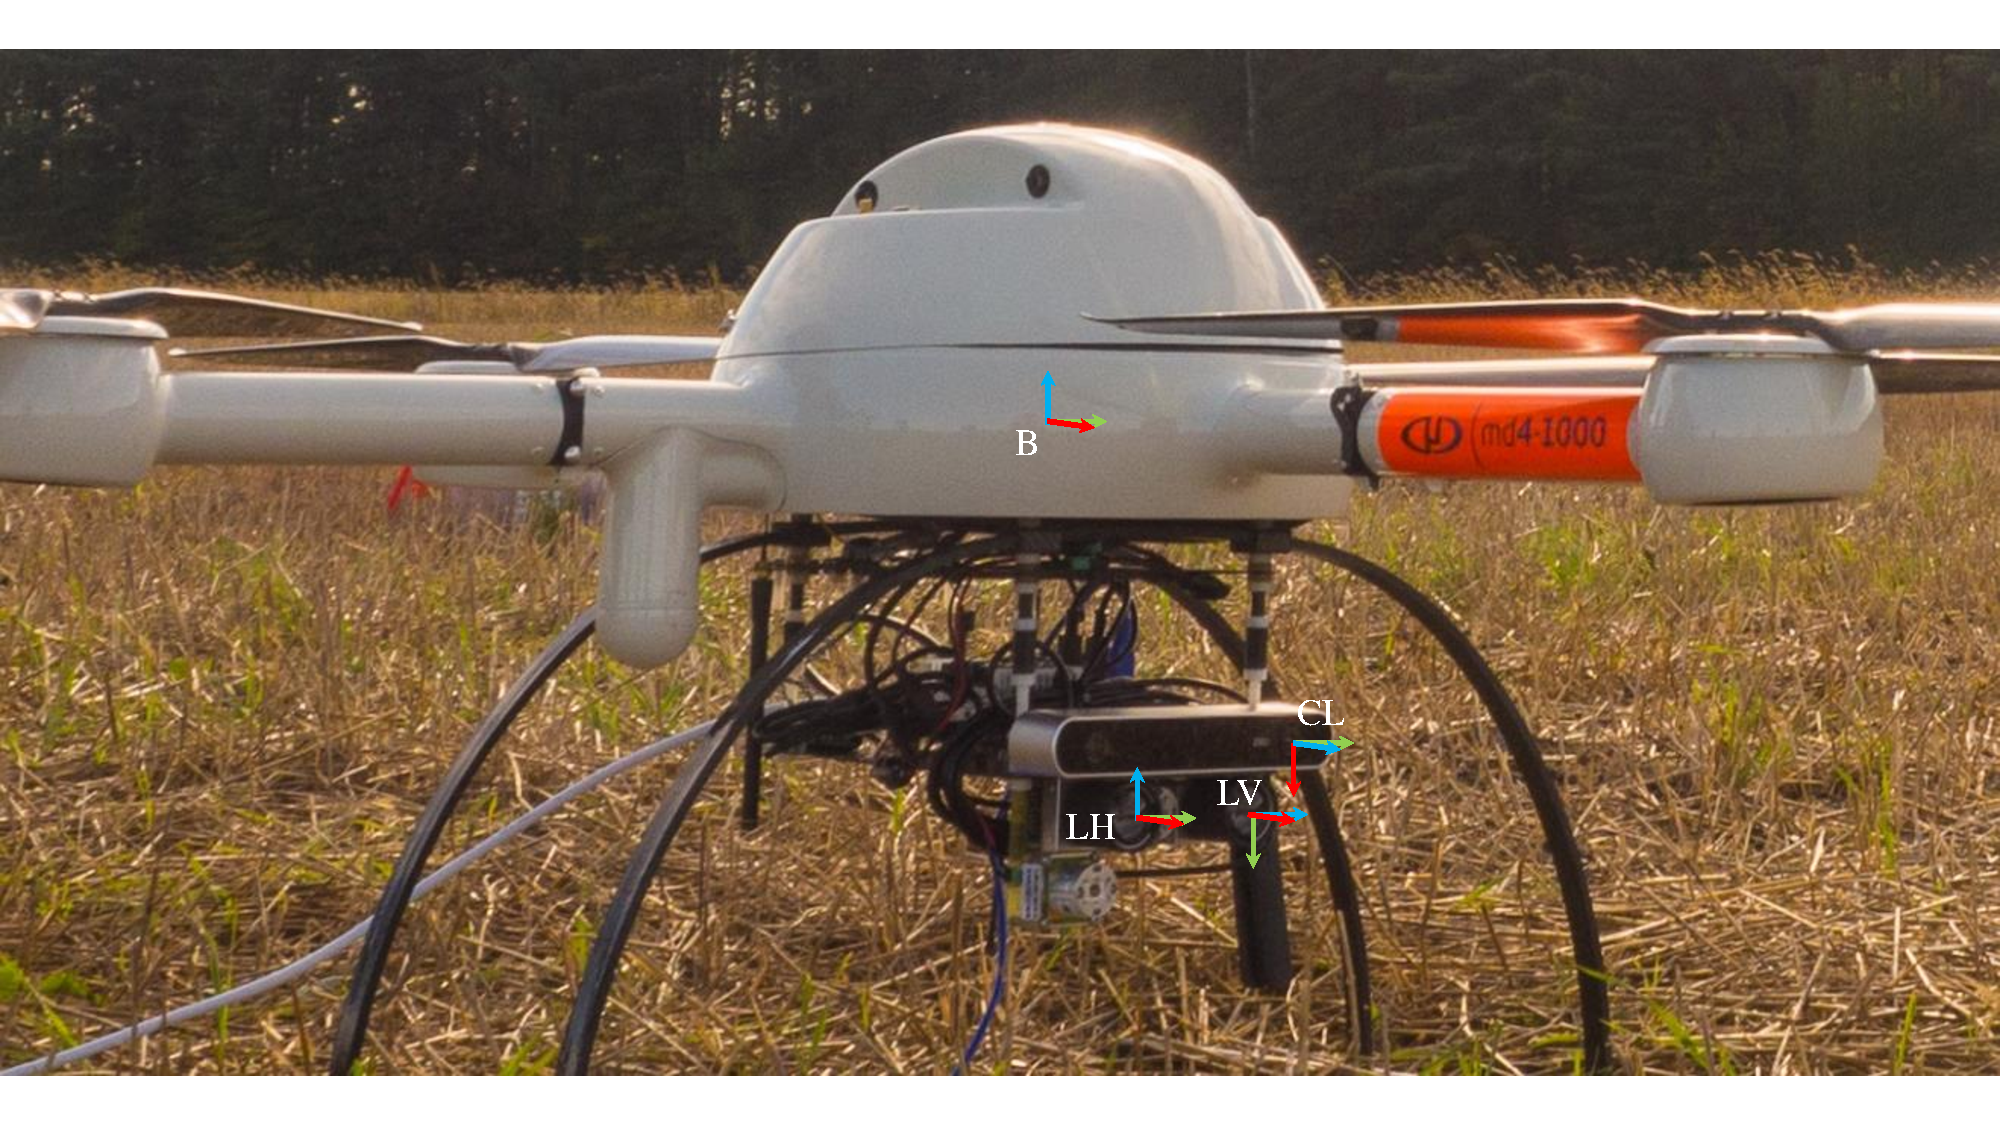
\includegraphics[width=0.95\linewidth]{images/md41000}
  \caption{Systèmes de coordonnées sur le md4-1000}
  \label{fig:md41000}
\end{figure}

\begin{table}[htp]
  \centering
  \setlength{\tabcolsep}{12pt}
  \begin{tabular}[htp]{|c|l|p{10cm}|}
    \hline
    Symbole & Nom                   & Description\\\hline
    $W$     &  \textit{World}       & Suivant la convention \textit{East-North-Up} (ENU), centrée au point de décollage du véhicule avec l'axe $x$ pointant vers l'Est, $y$ pointant vers le Nord et $z$ pointant vers le haut.\\ \hline
    $B$     &  \textit{Body}        & Encore suivant la convention ENU, l'axe $x$ pointant vers la droite, $y$ vers l'avant et $z$ vers le haut. \\ \hline
    $\mathit{BT}$  &  \textit{Body Tangent} & Repère centré sur, $B$ mais compensé pour ses angles de roulis et de tangage (mais pas de lacet). En d'autres mots, le repère ${BT}$ est donc tangent à la surface de la Terre et centré sur $B$. \\ \hline
    $\mathit{C[L,R]}$ & \textit{Camera} & Suivant la convention de représentation d'images, nous avons l'axe $x$ vers la droite, $y$ vers le bas et $z$ sortant de la caméra. Les suffixes $L$ et $R$ indiquent les caméras gauche et droite respectivement. Par souci de brièveté si le repère est écrit $C$ sans préciser la caméra gauche ou la caméra droite, il indique la caméra gauche.   \\ \hline
    $\mathit{L[H,V]}$ & \textit{Laser}& Les lasers aussi suivent un repère main droite avec $x$ vers l'avant, $y$ à gauche et $z$ vers le haut. Les données de distance du laser se situent toutes sur son plan $XY$. Les suffixes $H$ et $V$ indiquent la direction du balayage respectivement horizontal et vertical, par rapport au repère $B$. \\ \hline
    $\mathit{T}$ & \textit{Turbine} & Le système de coordonnées de la turbine est centré sur le rotor avec $x$ vers la droite (vu de devant), $y$ vers l'intérieur de la nacelle et $z$ vers le haut. \\ \hline
  \end{tabular}
  \setlength{\tabcolsep}{6pt}
  \caption{Repères présents dans le système d'inspection d'éoliennes}
  \label{table:coordinate_frames}
\end{table}

\section{Approche du rotor}

\subsection{Approche de loin avec caméra}
\label{subsec:approche_loin}

L'approche à longue distance comporte plusieurs avantages dont l'absence du besoin d'informations \textit{a priori} à propos du placement des pales. Avec une vue d'ensemble de l'éolienne à inspecter, il devient possible de mesurer l'angle des pales, une information cruciale qui sera exploitée lorsque l'UAV devra choisir où se diriger lorsqu'il est près du rotor. Le deuxième avantage est qu'il est possible de mesurer l'angle de lacet relatif entre l'UAV et l'éolienne, permettant ainsi de placer le véhicule perpendiculairement à la surface des pales. Cette méthode requiert tout de même la présence d'un détecteur de proximité avec une portée d'au moins 10 mètres; en revanche elle reste beaucoup moins dispendieuse que l'utilisation d'un scanner laser.

Dans cette section nous détaillons une méthode légèrement modifiée de celle de \citep{Stokkeland2015} pour détecter le centre du rotor d'une éolienne à partir d'une image. En somme, les étapes restent les mêmes, mais une robustesse additionnelle est introduite au moyen d'algorithmes de regroupement; une représentation différente des pales détectées est utilisée et un filtre de Kalman non linéaire (au lieu d'un filtre de Kalman linéaire) est proposé.

La méthode de détection du rotor se divise en 6 étapes et repose principalement sur des raisonnements géométriques,

\begin{enumerate}
  \item Prétraitement de l'image
  \item Détection de contours
  \item Détection de lignes
  \item Recherche de la tour
  \item Recherche des candidats de segments de pales
  \item Procédure de filtrage des candidats et calcul de la position du rotor
\end{enumerate}

%\begin{enumerate}
%  \item Prétraitement de l'image
%  \begin{enumerate}
%    \item Conversion de l'image couleur à une échelle de gris
%    \item Suppression du bruit par un filtre à convolution Gaussien
%    \item Correction du contraste par égalisation de l'histogramme
%  \end{enumerate}
%  \item Détection de contours par l'algorithme de Canny
%  \item Détection de lignes par transformée de Hough probabiliste
%  \item Trouver la tour de l'éolienne en cherchant des segments verticaux débutant au bas de l'image avec compensation de l'angle de roulis du véhicule.
%  \item Trouver les candidats de segments de pales. Ce sont les segments ayant un sommet près du plus haut point détectable de la tour.
%  \item Regroupement des segments par l'algorithme DBSCAN suivi du rejet de données aberrantes par une procédure de vote.
%  \item Moyenner les segments de pales et trouver le rotor par l'intersection du prolongement des pales.
%\end{enumerate}

\subsubsection{Étape 1: Prétraitement de l'image} Avant de commencer la détection, quelques corrections à l'image doivent être apportées. Puisque la procédure ne requiert pas de données de couleur, une conversion RGB en échelle de gris est effectuée au moyen de la transformée
\begin{align}
 Y \leftarrow 0.299 R + 0.587 G + 0.114 B
 \label{eq:rgb2gray}
\end{align}
où $Y$ est le niveau de gris du pixel entre $0$ et $255$ ce qui donne comme résultat l'image de la Figure \ref{fig:detection_pretraitement} (B). Les coefficients utilisés proviennent de la norme BT.601 de l'\cite{BT601Stu24online} pour le système d'encodage de couleurs YCbCr. En d'autres mots, nous effectuons une conversion de RGB à YCbCr mais nous ne gardons que le canal Y représentant la luminance. Pour éliminer la présence de bruit et atténuer les textures à haute fréquence pouvant donner lieu à une surdétection de lignes lors de la transformée de Hough, nous appliquons un filtre moyenneur $3 \times 3$ par convolution. Pour l'image floutée $F$, nous avons donc
\begin{align}
  F = \Bigg(\frac{1}{9}
    \begin{bmatrix}
      1 & 1 & 1\\
      1 & 1 & 1\\
      1 & 1 & 1
    \end{bmatrix}
  \Bigg) * H
  \label{eq:boxfilter}
\end{align}
avec le résultat visible à la Figure \ref{fig:detection_pretraitement} (C). Pour les convolutions sur les bords de l'image, nous répétons la valeur du pixel du bord pour les données manquantes dans l'opération de convolution. Pour augmenter le contraste et corriger les erreurs d'exposition de la caméra, une égalisation d'histogramme est appliquée. Pour l'image originale $I$ et l'image égalisée $H$ que l'on peut voir dans la Figure \ref{fig:detection_pretraitement} (D), nous avons
\begin{align}
  p_n &= \frac{\text{\# de pixels d'intensité } n }{\text{\# de pixels total}}, \ \ n = 0, \ldots, 255 \\
  H_{i,j} &= \text{floor}(255 \sum_{n=0}^{I_{i,j}} p_n)
  \label{eq:egalisation_histogramme}
\end{align}
où floor() est l'opérateur arrondissant à la baisse à l'entier le plus proche.
\begin{figure}[htp]
\centering
\begin{minipage}{0.49\textwidth}
  \centering
  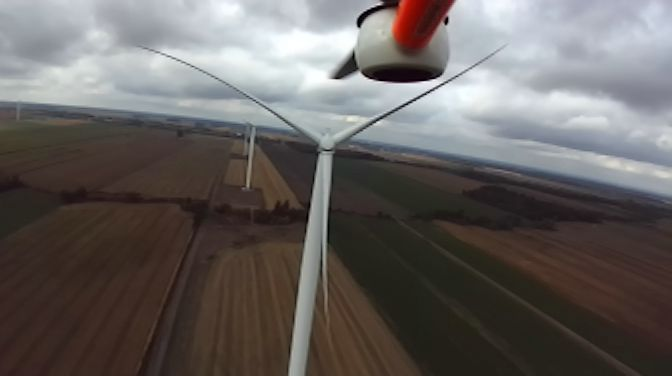
\includegraphics[width=\linewidth]{images/preprocess_original.png}
  (A)
\end{minipage}
\begin{minipage}{0.49\textwidth}
  \centering
  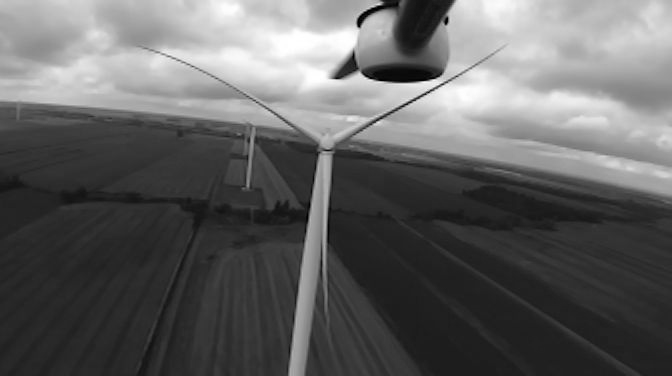
\includegraphics[width=\linewidth]{images/preprocess_gray.png}
  (B)
\end{minipage}
\vskip 1em
\begin{minipage}{0.49\textwidth}
  \centering
  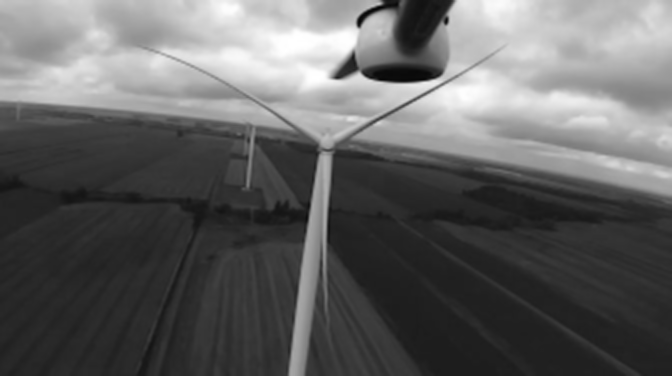
\includegraphics[width=\linewidth]{images/preprocess_blur.png}
  (C)
\end{minipage}
\begin{minipage}{0.49\textwidth}
  \centering
  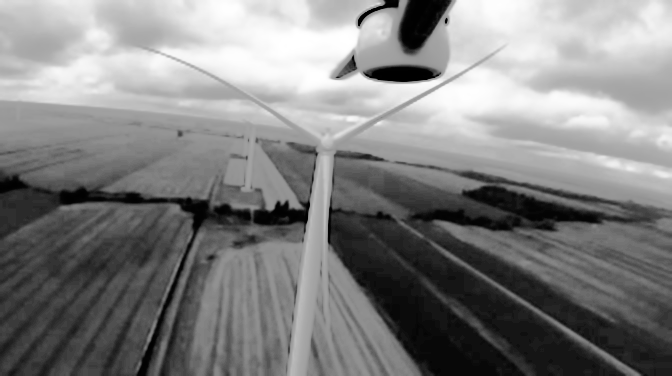
\includegraphics[width=\linewidth]{images/preprocess_histogram.png}
  (D)
\end{minipage}
\caption[Prétraitement d'image pour la détection de lignes.]{(A) Image originale (B) Image en tons de gris (C) Image floutée par un filtre moyenneur (D) Image avec égalisation d'histogramme.}
\label{fig:detection_pretraitement}
\end{figure}

\subsubsection{Étape 2: Détection de contours}
La détection de contours se fait au moyen de l'algorithme de \citep{Canny1986} et le résultat de la procédure est visible dans la Figure \ref{fig:canny}.

% qui à son tour se fait en une série de 4 étapes:
%
% \begin{enumerate}
%   \item Un filtre Gaussien par convolution est appliqué pour atténuer le bruit. Pour générer un masque Gaussien $H$ en deux dimensions il suffit de suivre l'équation:
%   \begin{align}
%     H_{ij}= \frac{1}{2\pi\sigma^2}\exp \left(-\frac{(i-(k+1))^2+(j-(k+1))^2}{2\sigma^2} \right) ; 1 \leq i, j \leq (2k + 1)
%   \end{align}
%   où $k$ est la taille du masque, $\sigma$ est l'écart type de la distribution et $i$ et $j$ sont les indexes de rangée et de colonne respectivement. Pour $k = 5$ et $\sigma = 1.4$ nous avons
%   \begin{align}
%     I_{\text{floue}} = \frac{1}{159} \begin{bmatrix}
%       2 & 4 & 5 & 4 & 2\\
%       4 & 9 & 12 & 9 & 4\\
%       5 & 12 & 15 & 12 & 5\\
%       4 & 9 & 12 & 9 & 4\\
%       2 & 4 & 5 & 4 & 2
%     \end{bmatrix} * I_{\text{originale}}
%   \end{align}
%   \item Pour chaque pixel le gradient $G$ et l'angle du gradient $\Theta$ est calculé à partir des quantitées $G_x$ le gradient horizontal et $G_y$ le gradient vertical suivant les équations:
%   \begin{align}
%     G_x =  \begin{bmatrix} -1 & 0 & 1 \\
%     -2 & 0 & 2 \\
%     -1 & 0 & 1
%   \end{bmatrix} * I_{\text{floue}}
%   \end{align}
%   \begin{align}
%     G_y = \begin{bmatrix}
%     -1 & -2 & -1\\
%     0 & 0 & 0 \\
%     1 & 2 & 1
%   \end{bmatrix} * I_{\text{floue}}
%   \end{align}
%   \begin{align}
%     G = \sqrt{G_x^2 + G_y^2}
%   \end{align}
%   \begin{align}
%     \Theta = \atantwo(G_y^2, G_x^2)
%   \end{align}
%   \item Une suppression des non-maxima est appliquée. Pour un pixel de l'image gradient $G_{ij}$ nous comparons la valeurs aux deux pixels adjacents dans les directions $\pm\Theta$, si la valeur de $G_{ij}$ est plus grande que les deux autres, il est gardé, sinon il est mit à $0$.
%   \item Un double seuil, l'un haut $T_h$ et l'autre bas $T_b$, est appliqué par hystérésis pour atténuer les pixels de contours trop faibles. Un pixel $G_{ij}$ plus fort que $T_h$ est marqué comme un pixel au contour fort. Les pixels plus faibles que $T_b$ sont supprimés (mise à $0$). Les pixels entre les deux sont gardés seulement s'ils sont adjacents à un pixel fort. Canny suggère que le ratio $T_b$ à $T_h$ soit entre $1:2$ et $1:3$.
% \end{enumerate}

\begin{figure}[htp]
  \centering
  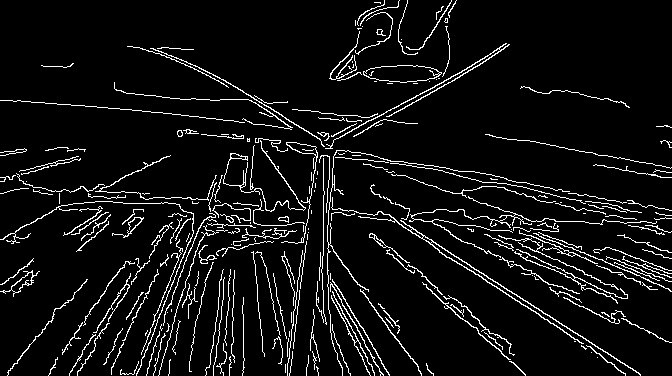
\includegraphics[width=0.6\linewidth]{images/canny.png}
  \caption{Résultat de l'application du filtre de Canny avec $T_b = 27$ et $T_h = 81$.}
  \label{fig:canny}
\end{figure}

Outre la méthode de Canny, il existe des méthodes modernes plus performantes que celle de Canny, par exemple \citep{Xie2015} proposent un réseau de neurones entièrement convolutionel capable de détecter beaucoup mieux les contours, et ce, sans avoir à manuellement ajuster ses paramètres. Par contre dans nos tests, la haute précision de la méthode retournait trop de contours, et il devenait difficile de passer aux prochaines étapes de la détection.

\subsubsection{Étape 3: Détection de lignes}

Une fois les contours trouvés, nous pouvons les utiliser pour détecter des segments de droite dans l'image. Dans le cas où des parties du véhicule sont visibles dans l'image, il suffit d'appliquer un masque avant de débuter cette étape. Nous appliquons la transformée de Hough probabiliste \citep{Matas2000} afin de détecter des segments de droites dans l'image de contours. Dans la Figure \ref{fig:detect_result_step6} tous les segments de couleur sont ceux détetectés par la transformée de Hough, la couleur reflète l'étape de sélection i.e. rouge pour l'étape 3, mauve pour l'étape 4, rose pour l'étape 5 et diverses couleurs pour chaque pale de l'étape 6.

\subsubsection{Étape 4: Recherche de la tour}
\label{subsubsec:approach4}

Stokkeland explique que la partie la plus facile à détecter est la tour puisqu'elle est toujours verticale et répond fortement à la détection de lignes. Pour la trouver, il suffit de chercher une ligne verticale (compensée pour l'angle de roulis de l'UAV) dont l'un des sommets repose dans la base de l'image. Puisqu'il arrive parfois que la détection de ligne défasse la tour en plusieurs segments, une fois le segment initial choisi, on recherche aussi des prolongements de ce segment à une certaine distance du plus haut sommet.

\subsubsection{Étape 5: Recherche des pales}

À la fin de l'étape 4, nous avons un ensemble de segments appartenant à la tour. À partir du plus haut point de ces segments, nous recherchons tout autre segment ayant un sommet dans un certain rayon du point. Ces segments sont considérés en tant que candidats à être des segments d'une pale.

Nous divergeons de la méthode proposée par Stokkeland où il tente de regrouper les segments selon l'angle par rapport à la tour au travers d'une procédure vorace simple où un nouveau groupe est créé lorsqu'un segment est à un angle au-dessus d'un certain seuil du groupe courant. Nous notons que ceci fonctionne acceptablement sur le jeu de données de Stokkeland où le ciel est clair et son éolienne est sur une colline près de la mer, mettant donc l'horizon bien en dessous du rotor. Lors de nos essais, tant en simulation que sur le terrain, nous avons noté que l'horizon était très proche du rotor, donnant lieu à une grande présence de segments près du rotor, faussant ainsi les résultats de la recherche de pales. C'est pourquoi nous implémentons l'étape 5 avec un algorithme de groupage formel qui inclut la résistance au bruit de mesure, nommé \textit{Density-based spatial clustering of applications with noise} (DBSCAN) proposée par \citep{Ester1996}.

La particularité de DBSCAN comparativement à d'autres algorithmes de partitionnement tel que $k$-means est que nous n'avons pas à fournir le nombre $k$ de partitions recherchées. À la place, nous ne fournissons que deux paramètres, $\epsilon$ (eps) la distance d'un point à son entourage, et MinPts le nombre minimum de points pour qu'une partition soit formée. Pour chaque segment, nous projetons leur angle par rapport à la tour sur un cercle unitaire. Ceci permet d'exécuter DBSCAN dans un espace euclidien pour regrouper les segments adjacents.

Une fois les groupes formés, Stokkeland utilise une stratégie de vote pour éliminer les fausses détections. La moyenne des angles est calculée et une procédure de vote débute s'il y a plus de deux groupes. Nous en choisissons deux au lieu de trois tel que proposé par Stokkeland pour prendre en compte le cas où une pale est vis-à-vis la tour. Sachant que les éoliennes ont toujours trois pales espacées de $120$ degrés, chaque groupe calcule sa distance angulaire par rapport aux autres et vote pour les groupes n'étant pas à $120$ degrés d’eux-mêmes. Dans le cas où DBSCAN ne ressort que deux groupes, la direction de la troisième pale est approximée à 120 degrés des deux autres pales.

\subsubsection{Étape 6: Recherche du rotor et filtrage}

L'étape 5 nous a donc fourni trois groupes de segments représentant chacun les pales de l'éolienne. Le centre du rotor peut donc être calculé en moyennant chaque groupe puis en prenant la moyenne de l'intersection des prolongements de chaque segment.

\begin{figure}[htb]
  \centering
  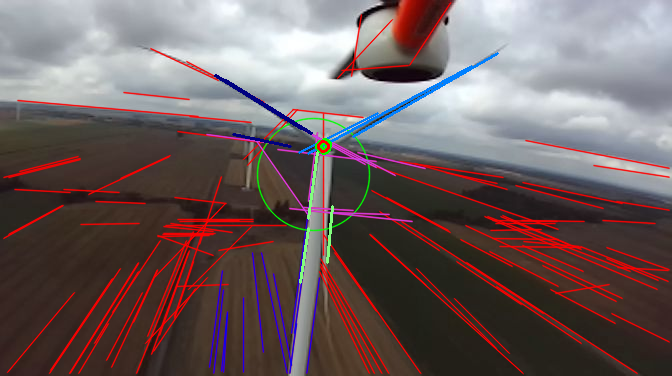
\includegraphics[width=0.8\linewidth]{images/turbine_detect_result.png}
  \caption{Résultat d'une détection réussie à la fin de la procédure.}
  \label{fig:detect_result_step6}
\end{figure}

Dans la Figure \ref{fig:detect_result_step6}, nous pouvons observer les étapes $3$ à $6$ en opération. Toutes les lignes sont le résultat de la transformée de Hough appliquée à l'image des bordures suite à l'application de l'algorithme de Canny. Au bas de l'image, les lignes mauves sont les candidates à être des lignes de la tour. Elles se font rejeter car elles ne s'étendent pas assez haut dans l'image. Le grand cercle vert est celui tracé au plus haut point de la tour dans lequel les segments de pales sont recherchés. Les segments roses sont les candidats de pales rejetés par l'algorithme de partitionnement DBSCAN et la procédure de vote.
%C'est ici que nous voyons l'amélioration de l'algorithme par rapport à Stokkeland où malgré la grande quantité de segments provenant de l'arrière plan, les pales sont quand même bien choisies.
Les pales finales sont indiquées par les lignes bleu, bleu foncé et vert pâle. Finalement, avec l'application des étapes $5$ et $6$ on peut voir que l'intersection des pales se croise bien sur le centre du rotor.

Le point détecté passe ensuite dans un filtre de Kalman linéaire permettant ainsi de garder une estimation de la position du rotor dans l'image lorsque la détection échoue. Le vecteur d'état $\vect{x}_k$ contient la position et la vitesse de déplacement en coordonnées image du centre du rotor. La matrice de transition $\vect{F}_k$ contient les termes $\gamma_x, \gamma_y \in [0, 1]$ faisant décroître la vitesse exponentiellement avec le temps. Ceci empêche l'estimation de diverger à l'infini quand aucune mesure n'entre dans le filtre pendant de longues périodes de temps.
\begin{align}
  \begin{sbmatrix}{\boldsymbol{x}_k}u(k) \\ v(k) \\ \dot{u}(k) \\ \dot{v}(k)\end{sbmatrix} =
  \begin{sbmatrix}{\boldsymbol{F}_k}
    1 & 0 & 1 & 0\\
    0 & 1 & 0 & 1\\
    0 & 0 &  \gamma_x & 0\\
    0 & 0 & 0 &  \gamma_y
  \end{sbmatrix} \begin{sbmatrix}{\boldsymbol{x}_{k-1}}u(k-1) \\ v(k-1) \\ \dot{u}(k-1) \\ \dot{v}(k-1)\end{sbmatrix}
  + \boldsymbol{w}_k
\end{align}
où $\boldsymbol{w}_k$ est un bruit blanc gaussien. Le modèle de mesure inclut seulement la détection du point dans l'image.
\begin{align}
  \begin{sbmatrix}{\boldsymbol{z}_k}z_x \\ z_y\end{sbmatrix} =
  \begin{sbmatrix}{\boldsymbol{H}_k}
    1 & 0 & 0 & 0\\
    0 & 1 & 0 & 0
  \end{sbmatrix} \begin{sbmatrix}{\boldsymbol{x}_{k}}u(k) \\ v(k) \\ \dot{u}(k) \\ \dot{v}(k)\end{sbmatrix}
  + \boldsymbol{v}_k
\end{align}
Le terme d'entrée de commande $\boldsymbol{u}_k$ pourrait être utilisé pour prendre en compte les vitesses angulaires commandées au robot. Par contre sachant qu'elles ne seront pas disponibles sur le lien de télémétrie du md4-1000, nous ne les prenons pas en compte. La meilleure façon d'améliorer le filtre serait d'ajouter des mesures de $\dot{u}$ et de $\dot{v}$, chose qui pourrait être faite par des méthodes de calcul de flux optique.

Une fois le point $(u,v)$ trouvé dans l'image, il suffit d'appliquer le modèle de caméra sténopé de la section \ref{subsec:modele_camera} et sa matrice de paramètres intrinsèques $K$ pour obtenir un vecteur unitaire $u_C$ dans le repère caméra pointant vers le rotor. Puisque la distance entre l'UAV et le rotor est beaucoup plus grande que la distance entre la caméra ($C$) et le centre du véhicule ($B$) nous pouvons la négliger. Ce qui implique que nous pouvons appliquer quelques rotations pour remettre ce vecteur unitaire dans le système d'axes $W$ (centré sur $B$) à partir de $C$ pour obtenir $\vect{u}_W$. En supposant que le point $(u,v)$ provient de l'image rectifié il suffit de suivre l'équation suivante:
\begin{align}
  \vect{u}^W = \vect{R}^W_B \vect{R}^B_C \vect{u}^C = \vect{R}^W_B \vect{R}^B_C \vect{K}^{-1} \begin{bmatrix}u \\ v \\ 1\end{bmatrix}
\end{align}
où $\vect{K}$ est la matrice des paramètres intrinsèques (eq. \ref{eq:intrinsics}). Pour se rendre au rotor, il suffit donc de commander une vitesse dans la direction $\vect{u}^W$. Puisque nous n'avons pas de mesure de distance entre l'éolienne et l'UAV, la vitesse demeure constante; elle peut être régulée que lorsque la surface entre dans la portée du capteur de proximité.

\subsection{Approche en remontant la tour}
\label{subsec:laser_tower}

Dans cette méthode le véhicule est placé à proximité de la tour de telle sorte que le scanner laser puisse capter la forme de la tour et de la discontinuité introduite à l'endroit où la tour rencontre le rotor. Cette méthode est plus simple et plus fiable que l'approche visuelle, mais elle repose sur deux hypothèses:
\begin{enumerate}
  \item Le véhicule est bien placé par l'opérateur devant l'éolienne de telle sorte que les capteurs soient perpendiculaires au plan sur lequel les pales reposent.
  \item Aucune pale n'est placée devant la tour, et l'angle de chaque pale est connu d'avance.
\end{enumerate}

Le principe opérationnel est simple et illustré dans la Figure \ref{fig:approach}. Le scanner laser horizontal est utilisé pour centrer l'UAV devant la tour et garder une distance de sécurité alors que le scanner vertical est utilisé pour détecter le rotor. Pour ce faire, il faut tout d'abord projeter les mesures de distances à un nuage de points 3D au moyen de l'équation \ref{eq:scan2cloud} où $r_i$ est une distance, $\theta_i$ l'angle correspondant à la mesure $i$, et $n$ le nombre de mesures retournées par le laser. Nous notons que cette méthode requiert peu de mesures laser et donc il n'y a pas besoin d'un lidar sophistiqué. Par exemple le lidar que nous utilisons ne fourni que huit mesures.
\begin{align}
  {\vect{p}_{L}}_i = \begin{bmatrix}
    p^L_{i_x} \\
    p^L_{i_y} \\
    p^L_{i_z}
  \end{bmatrix} = \begin{bmatrix}r_i \cos \theta_i \\ r_i \sin \theta_i \\ 0 \end{bmatrix} & \text{ où } i=1,\ldots,n
    \label{eq:scan2cloud}
\end{align}
\begin{figure}[htp]
  \centering
  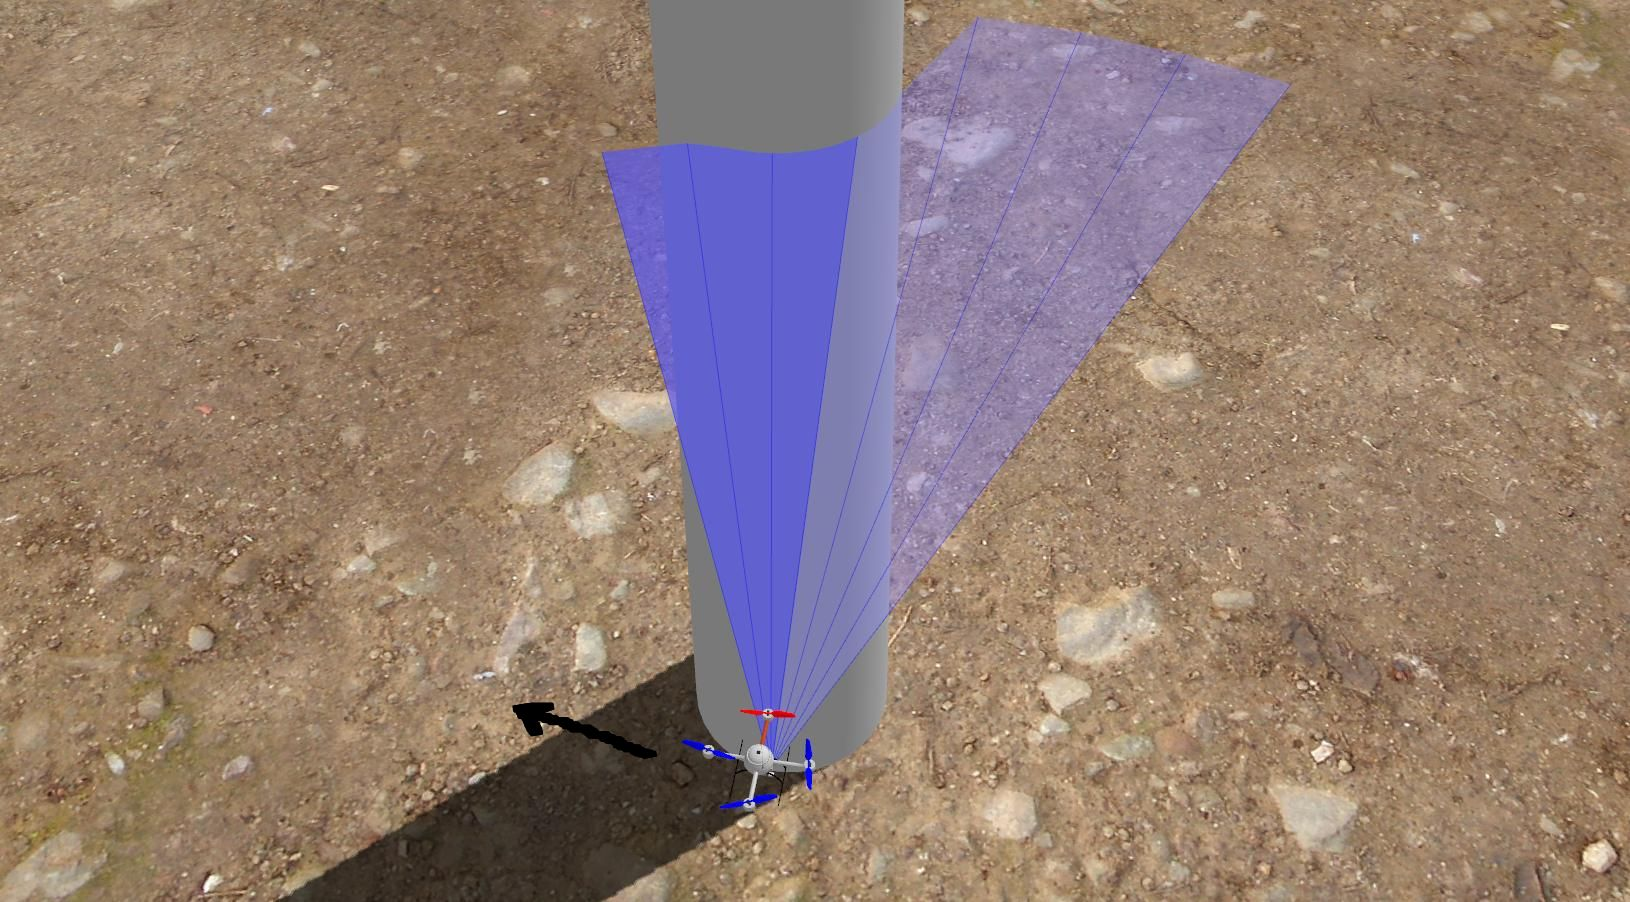
\includegraphics[width=0.8\linewidth]{images/principe_operation.jpg}
  \caption{Principe d'opération de l'approche du rotor par laser.}
  \label{fig:approach}
\end{figure}
L'équation \ref{eq:scan2cloud} nous donne des points dans le repère du laser correspondant, puisque les matrices de transformées homogènes $\vect{T}_{LH}^B$, $\vect{T}_{LV}^B$ ainsi que la rotation $\vect{R}_B^{BT}$ sont connues, il suffit de transformer chaque $\vect{p}^L$ au repère ${BT}$ suivant l'équation \ref{eq:pointcloud_bodytangent}.
\begin{align}
  \begin{bmatrix}\vect{p}^{BT}_i \\ 1\end{bmatrix} = \begin{bmatrix}
    \vect{R}_B^{BT} & 0 \\
    0 & 1
  \end{bmatrix} \vect{T}_{L}^B\begin{bmatrix}\vect{p}^{L}_i \\ 1\end{bmatrix}
  \label{eq:pointcloud_bodytangent}
\end{align}

Une fois ces mesures transformées dans le bon repère, nous pouvons appliquer une loi de contrôle de type PID sur les axes $x$ et $y$ en plus d'une vitesse constante $v_z$ en $z$ pour calculer la commande de vitesse $\vect{v}(t)$ dans le repère ${BT}$ à envoyer à l'UAV tel que présenté dans l'équation \ref{eq:tower_pid}.

\begin{align}
  \vect{v}(t) = \begin{bmatrix}v_x(t)\\ v_y(t)\\ v_z(t)\end{bmatrix} =
  \begin{bmatrix}{K_p}_x e_x(t)\\ {K_p}_y e_y(t)\\ v_z\end{bmatrix} +
  \begin{bmatrix}{K_i}_x \int e_x dt\\ {K_i}_y \int e_y dt\\ 0\end{bmatrix} +
  \begin{bmatrix}{K_d}_x \dot{e}_x(t)\\ {K_d}_y \dot{e}_y(t)\\ 0\end{bmatrix}
  \label{eq:tower_pid}
\end{align}
\begin{align}
  e_x = \frac{1}{n} \sum_{i = 1}^n p^{BT}_{i_x}
  \label{eq:error_x}
\end{align}
\begin{align}
  e_y = d - {\text{min}}({p^{BT}_{i_y}})
  \label{eq:error_y}
\end{align}

L'équation \ref{eq:error_x} présente le terme d'erreur $e_x$ calculé en moyennant la composante $x$ des points ${p_{BT}}_i$ provenant du laser horizontal pour déterminer si l'UAV doit bouger vers sa gauche ou sa droite pour se centrer devant la tour. L'équation \ref{eq:error_y} présente le terme d'erreur $e_y$ qui prend la plus petite mesure en $y$ pour connaître la distance par rapport à la surface de la tour et $d$ est la distance de sécurité à garder par rapport à la tour.

La détection du rotor se fait au moyen d'une détection de discontinuité en faisant une convolution (voir l'équation \ref{eq:gaussian_derivative_conv}) de la composante $y$ des points du laser vertical avec un filtre à dérivée de gaussienne $\Gamma(x)$ discrétisé sur $n$ points dans le domaine $x \in [-5\sigma,5\sigma]$ généré par l'équation \ref{eq:gaussian_derivative}. Une discontinuité est détectée si la réponse $r$ du filtre est plus haut qu'un certain seuil à déterminer de façon empirique.
\begin{align}
  \vect{\Gamma}(x) = - \frac{x}{\sigma^3 \sqrt{2\pi}} \exp\left(\frac{-x^2}{2 \sigma^2}\right)
  \label{eq:gaussian_derivative}
\end{align}
\begin{align}
  r = {p^{BT}_y} * \vect{\Gamma}(x),
  \label{eq:gaussian_derivative_conv}
\end{align}
Pour contrer le bruit de mesure et s'assurer que la détection est valide, le véhicule ne s'arrête que si la détection s'active plusieurs fois dans un certain laps de temps.
%Un exemple de résultat en simulation est démontré dans la Figure \ref{fig:step_result}.
Le masque de convolution est de taille $1\times8$ et $\sigma = 0.5$.

%\begin{figure}[htp]
%  \centering
%  \begin{minipage}{0.4\textwidth}
%    \centering
%    
\includegraphics[width=\linewidth]{images/placeholder.png}
%  \end{minipage}
%  \begin{minipage}{0.4\textwidth}
%    \centering
%    
\includegraphics[width=\linewidth]{images/placeholder.png}
%  \end{minipage}
%  \caption{Résultat de la convolution sur un exemple de mesure.}
%  \label{fig:step_result}
%\end{figure}

\section{Suivi des pales}

Une fois devant le rotor, le véhicule utilise l'information sur l'angle des pales acquise au préalable (visuellement ou par entrée utilisateur) pour savoir dans quelle direction se diriger. Il est important à cette étape de garder une grande distance de sécurité ($d_{grand} = 8$ m ou plus) du rotor puisque celui-ci, constitué de multiples lignes électriques haute tension et d'une grande quantité de métal, peut causer de l'interférence magnétique avec le magnétomètre de l'UAV qui peut potentiellement résulter en une perte de l'orientation. Cette distance peut être diminuée à $d_{petit} = 4$ m lors du suivi une fois que le véhicule commence à s'éloigner du rotor.

Dans l'étape de suivi des pales, le principe est similaire à la montée de la tour. Le robot cherche à suivre la pale à une vitesse constante tout en restant à une distance désirée de la pale. Nous présentons deux approches possibles, la première dans la Section \ref{subsec:pcl_blade} par nuage de points applicable à des scanners lasers 3D ou un capteur par vision active, la deuxième dans la Section \ref{subsec:laser_blade} n'usant que des scanners lasers 2D.
%et la troisième dans la Section \ref{subsec:visual_blade} fonctionnant que visuellement.
Suivant la machine à états de la mission, une fois la fin de la pale détectée, le robot revient aux coordonnées GPS où le rotor a été détecté initialement. Puisque les pales d'une éolienne sont droites ou courbées vers l'avant, une trajectoire en ligne droite entre la fin de la pale et le devant du rotor est garantie d'être libre d'obstacles.

\subsection{Suivi par nuage de points}
\label{subsec:pcl_blade}

Dans cette méthode, nous reprenons l'algorithme proposé dans le Chapitre \ref{sec:ugv} pour le suivi de mur par UGV. L'algorithme est d'ailleurs plus simple puisqu'il n'y a aucun sol à filtrer du nuage de points. Cependant l'avantage majeur de cette méthode est qu’avec le calcul de la normale de la surface il devient possible de toujours placer le véhicule perpendiculaire à celle-ci, améliorant ainsi la qualité des images prises pendant l'inspection.

\begin{figure}[htp]
  \centering
  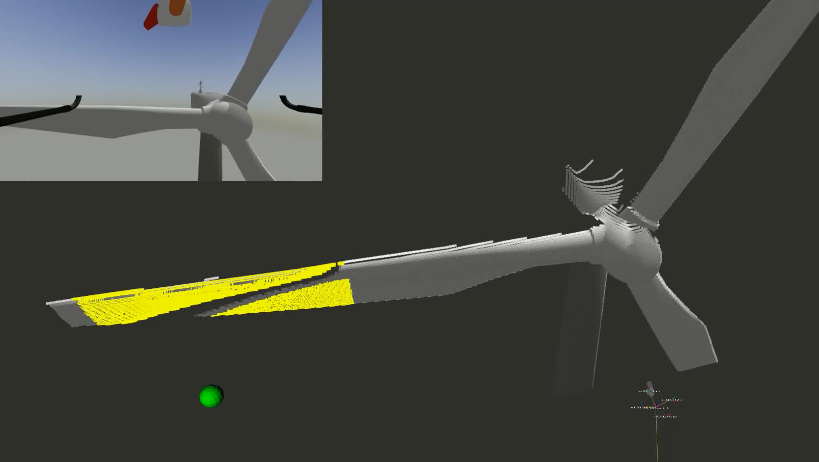
\includegraphics[width=0.7\linewidth]{images/suivit_nuage_points.png}
  \caption{Exemple de suivi de pale par nuage de points.}
  \label{fig:pcl_blade_follow}
\end{figure}

Le bout de la pale est détectée de la même façon qu'un mur à angle aigu est détecté dans la section \ref{sec:perimeter_exploration}. À mesure que le véhicule avance vers le bout de la pale, le nuage de points $\mathcal{S}$ devient de plus en plus petit, ainsi il devient possible de détecter le bout une fois que $\mathcal{S}$ passe un certain seuil. Dans la Figure \ref{fig:pcl_blade_follow}, les points blancs sont le nuage de points perçu par l'UAV alors que les points jaunes représentent la tranche sélectionnée $\mathcal{S}$. La boule verte est la commande de position envoyée à l'UAV, perpendiculaire à $\mathcal{S}$.

\subsection{Suivi par scanner laser 2D}
\label{subsec:laser_blade}

Le suivi par scanner laser se fait de la même façon que la montée de la tour au moyen de deux scanners lasers perpendiculaires l'un à l'autre. Suivant les mêmes formules de projection 2D à 3D présentées dans la section \ref{subsec:laser_tower}, le véhicule tente de se centrer par rapport à la pale en moyennant les points du nuage résultant tout en appliquant une vitesse constante $V_C$ dans la direction estimée de suivie. Dépendamment de l'angle de la pale seulement l'un des deux lasers est utilisé pour le suivi.

La loi de commande est donc encore un PID où les termes d'erreurs sont calculés à partir de la projection laser et la sortie est une commande de vitesse dans le repère ${BT}$.
\begin{align}
  \vect{u}(t) = \vect{V}_C(t) + \vect{K}_P \vect{e}(t) + \vect{K}_I\int{\vect{e}(t)dt} + \vect{K}_D\dot{e}(t)
  \label{eq:pid_laser_blade}
\end{align}
L'erreur $\vect{e}(t)$ est calculée différemment selon la direction de la pale. En pratique, on peut utiliser la moyenne du laser horizontal si la pale est à $\pm15^{\circ}$ de la verticale et le laser vertical dans tous les autres cas. Pour une pale horizontale nous aurions par exemple
\[
\vect{e}(t) = \begin{bmatrix}e_x(t) \\ e_y(t) \\ e_z(t)\end{bmatrix} =
\begin{bmatrix}
0 \\ d - \min(p^{BT}_{i_y}) \\ \frac{1}{n}\sum_{i=1}^{n}p^{BT}_{i_z}
\end{bmatrix} \text{ avec } i=1,\ldots,n
\]
Dans le cas où une erreur de capteur survient, par exemple si la pale devient assez mince pour passer entre deux rayons du laser, on répète la commande de vitesse précédente $\vect{u}(t) = \vect{u}(t-1)$. Ceci implique qu'une fois que le véhicule passe le bout de la pale, il continuera à voler dans le vide. La détection de bout de pale se fait donc aisément en comptant le nombre de lectures vides dans un certain laps de temps avec un seuil à ajuster en prenant en compte que des lectures vides peuvent survenir pendant le suivi de la pale.

% \subsection{Suivit visuel pur}
% \label{subsec:visual_blade}
%
% \color{red}
% XXX drop this section?
% \color{black}

\clearpage
\section{Implémentation}

Pour l'implémentation, la majorité de l'effort de développement a été dédiée à l'approche purement par scanner laser suivant les sections \ref{subsec:laser_tower} et \ref{subsec:laser_blade} puisqu'elles s'avèrent être les plus fiables, dépendent de moins de paramètres à ajuster manuellement, et sont peut coûteuses en termes de matériel comparé à une approche par scanner laser 3D. Le suivi par nuage de point de la section \ref{subsec:pcl_blade} a aussi été implémenté séparément pour nous permettre de vérifier la possibilité d'utiliser un capteur de profondeur. Cependant, nous posons l'hypothèse que cette méthode ne fonctionnerait pas avec une caméra stéréo dû à la surface sans texture de l'éolienne ni avec un capteur fonctionnant par \textit{Time of Flight} de par leur portée limitée.
%Nous prouverons plus tard tant en simulation que sur le terrain qu'une approche par camera stereo n'est pas viable pour ce problème.
De plus, nous implémentons aussi la méthode de Stokkeland modifiée décrite à la section \ref{subsec:approche_loin} pour la détection du rotor, mais à la vue des mauvais résultats obtenus nous n'avons pas poursuivi l'implémentation du contrôleur correspondant.

La simulation est donc développée en prévision d'un quadricoptère md4-1000 de Microdrones équipé de deux lidars LeddarVu8 de LeddarTech, une caméra stéréo Zed de ZedLabs et un ordinateur de bord Nvidia TX2. Les lidars Vu8 ont été sélectionnés avec un angle de vue de $48^{\circ}$ et ont la propriété particulière d'émettre des segments au lieu de faisceaux colmatés à la façon des lidars traditionnels. Par conséquent, il devient improbable en pratique qu'une pale d'éolienne puisse se perdre entre deux rayons du lidar.

%Le md4-1000 possède une interface de communication mdSI$^{2}$ (\textit{System Integrator Interface}) permettant de recevoir la télémétrie du robot et de lui envoyer des commandes de vitesse dans le repère $BT$.
L'intégralité du logiciel a été développé en C++ à l'aide de l'interlogiciel
Robot Operating System (ROS) incluant les pilotes pour les divers capteurs et la communication par UART au md4-1000. Le traitement d'images repose sur la librairie OpenCV \citep{itseez2015} et la machine à états faisant la gestion de la mission, présentée dans l'annexe \ref{annexe:state_machine}, a été écrite à l'aide de la librairie Boost \textit{Meta State Machine} \citep{Schling2011}. En tout temps, la machine, que l'on nomme \code{Commander} garde un pointeur vers un objet implémentant l'interface \code{ControllerInterface}. Ces contrôleurs sont instanciés et détruits dynamiquement à chaque changement d'état, nous permettant ainsi d'avoir accès à une grande quantité de contrôleurs spécifiques tout en gardant l'utilisation de la mémoire vive à un minimum. Le \code{Commander} calcule les commandes de vitesse à une fréquence de $50$Hz, la même que la fréquence maximale de l'odométrie. Quand une mise à jour d'odométrie ou des lidars est reçue, elle est mise dans un tampon en attente du prochain cycle de calcul.

\begin{figure}[htbp]
  \centering
  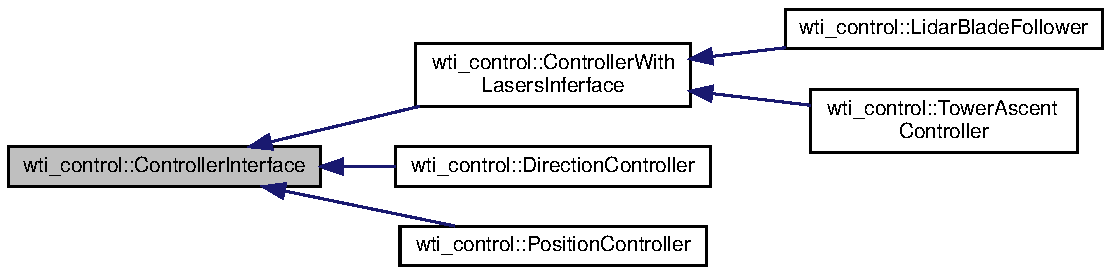
\includegraphics[width=\linewidth]{images/uml_controller.pdf}
  \caption{Diagramme de classe des différents contrôleurs utilisés par la machine à états.}
  \label{fig:uml_controller}
\end{figure}

La Figure \ref{fig:uml_controller} présente les contrôleurs utilisés dans le logiciel. Nous avons en particulier le \code{PositionController} pour la phase de retour au rotor, le \code{LidarBladeFollower} pour le suivi de pale et le \code{TowerAscentController} pour la montée de la tour. Le \code{DirectionController} n'est utilisé que pendant de courts instants de contrôle en boucle ouverte, par exemple la man\oe uvre pour éviter la zone d'interférence magnétique devant la nacelle.

\subsection{Résultats en simulation}
\label{subsec:results_simu}
La simulation se base sur celle pour véhicules multi rotors nommée RotorS développée par \citep{Furrer2016} dans l'environnement Gazebo\footnote{http://gazebosim.org}. Puisque le micrologiciel effectuant le contrôle de vol dans les véhicules de Microdrones demeure un secret industriel la simulation a été développée au moyen de véhicules déjà présents dans RotorS.
%Le contrôleur est donc basé sur celui de \citep{lee2010}, puisque celui-ci prend des commandes de position, vitesse et d'accélération additive d'un coup, nous pouvons simuler l'interface du md4-1000 en inscrivant la position et une accélération additive nulle dans la commande.
Le but n'est donc pas de réaliser une simulation précise de la physique du véhicule. On se concentre plutôt sur la simulation des capteurs et des comportements autonomes de haut niveau.

\begin{figure}[htp]
  \centering
    \centering
    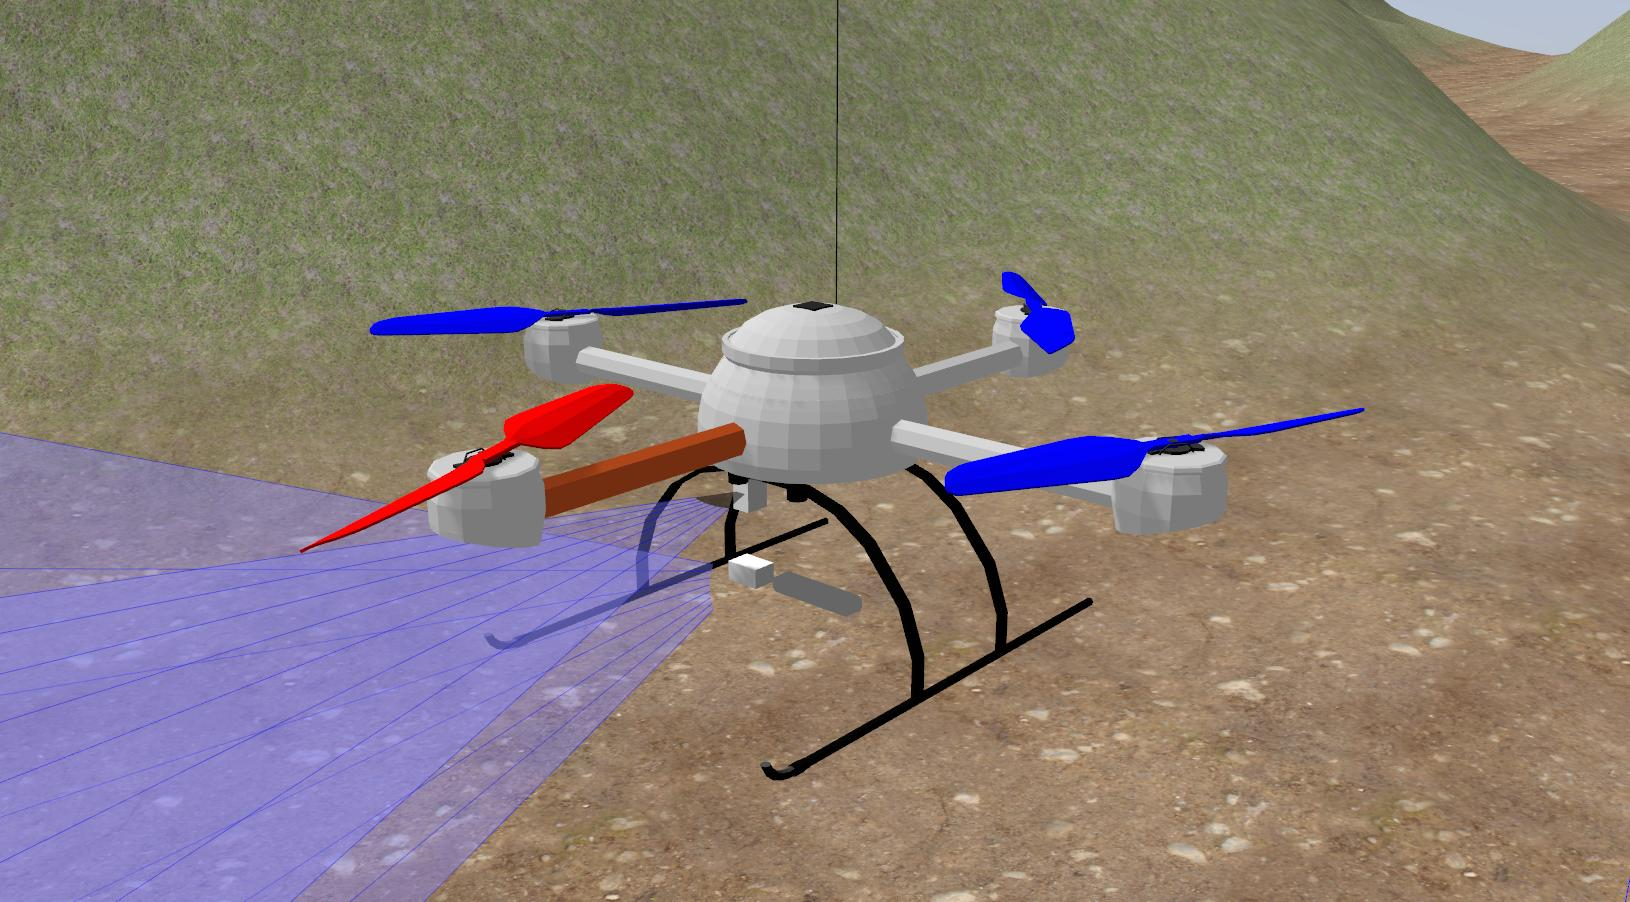
\includegraphics[width=0.7\linewidth]{images/sim_vehicle_closeup.jpg}
  \caption{Véhicule md4-1000 en simulation. Les rayons bleus sont les rayons projetés par les scanner lasers LeddarVu8.}
  \label{fig:sim_vehicle_closeup}
\end{figure}

Plusieurs environnements ont été implémentés incluant un monde simulant un parc éolien avec plusieurs éoliennes alignées (Figure \ref{fig:sim_worlds} (B)) et un monde avec une seule éolienne avec un montagne au loin (Figure \ref{fig:sim_worlds} (A)). La simulation suit le pire cas possible d'un parc éolien respectant les consignes du Département de l'Environnement du Royaume-Uni demandant un minimum de trois diamètres de rotor d'espacement entre chaque éolienne \citep{DOE2009}. Il faut noter que suite à des discussions avec des travailleurs de l'industrie, l'un des défauts de la simulation est que les pales des éoliennes sont normalement inclinées vers l'arrière de telle sorte qu'elles sont parallèles au sens du vent. Ceci permet au rotor de rester stationnaire lors des inspections. Notre algorithme reste toujours valide mais elle ne permet que d'inspecter le bord d'attaque des pales.

\begin{figure}[htbp]
  \centering
  \begin{minipage}{0.49\textwidth}
    \centering
    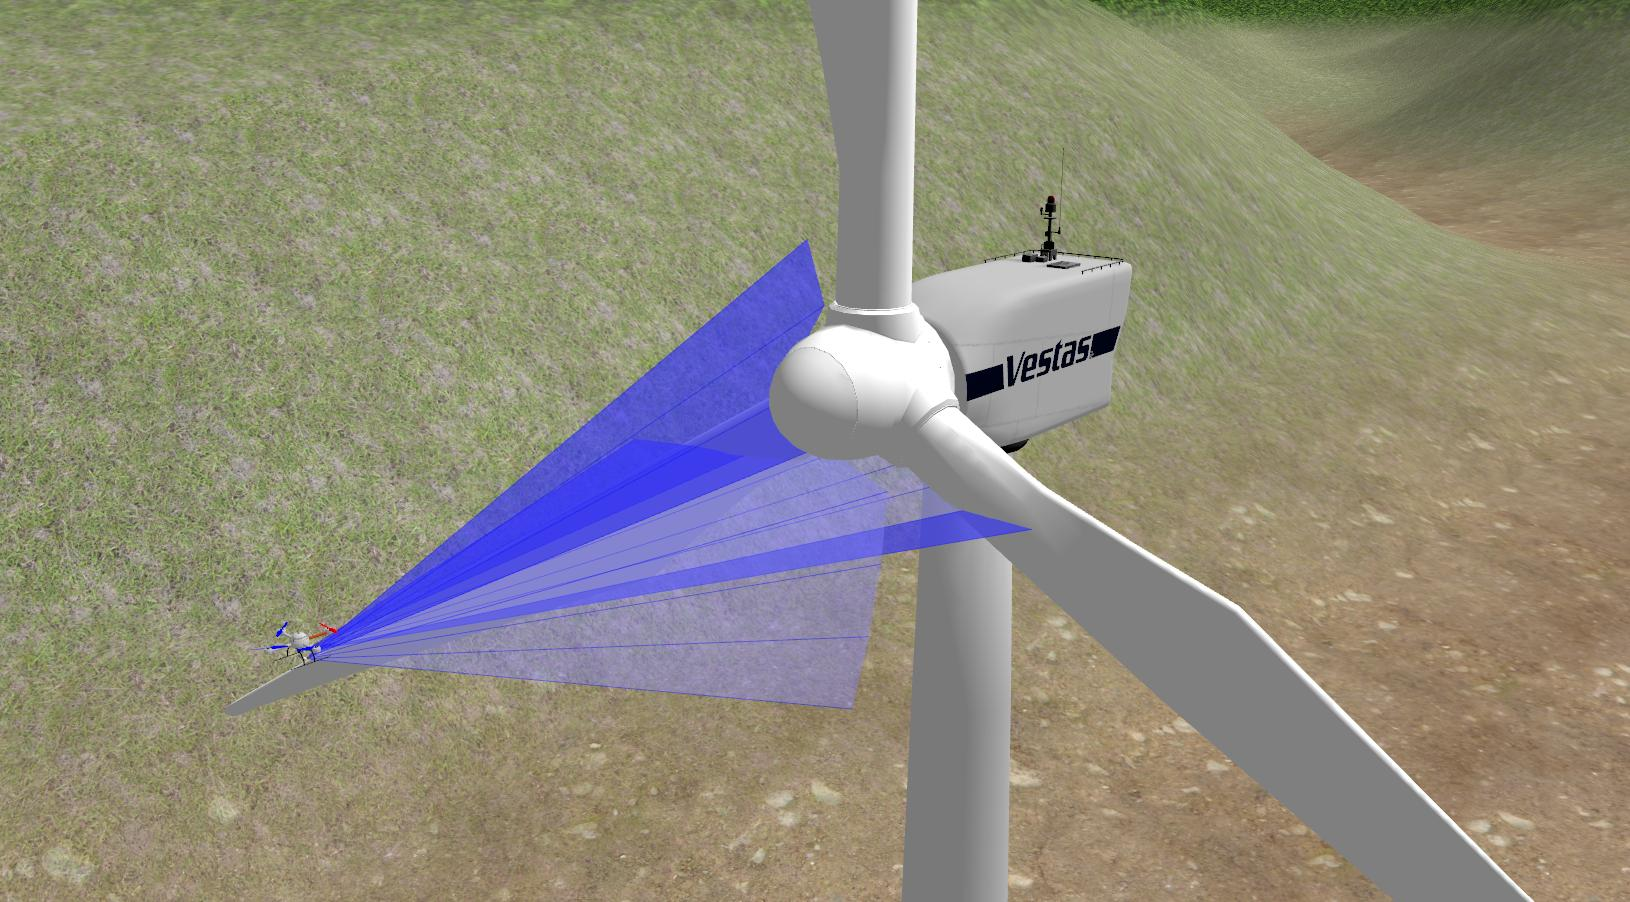
\includegraphics[width=\linewidth]{images/sim_vestas_closeup.jpg}
    (A)
  \end{minipage}
  \begin{minipage}{0.49\textwidth}
    \centering
    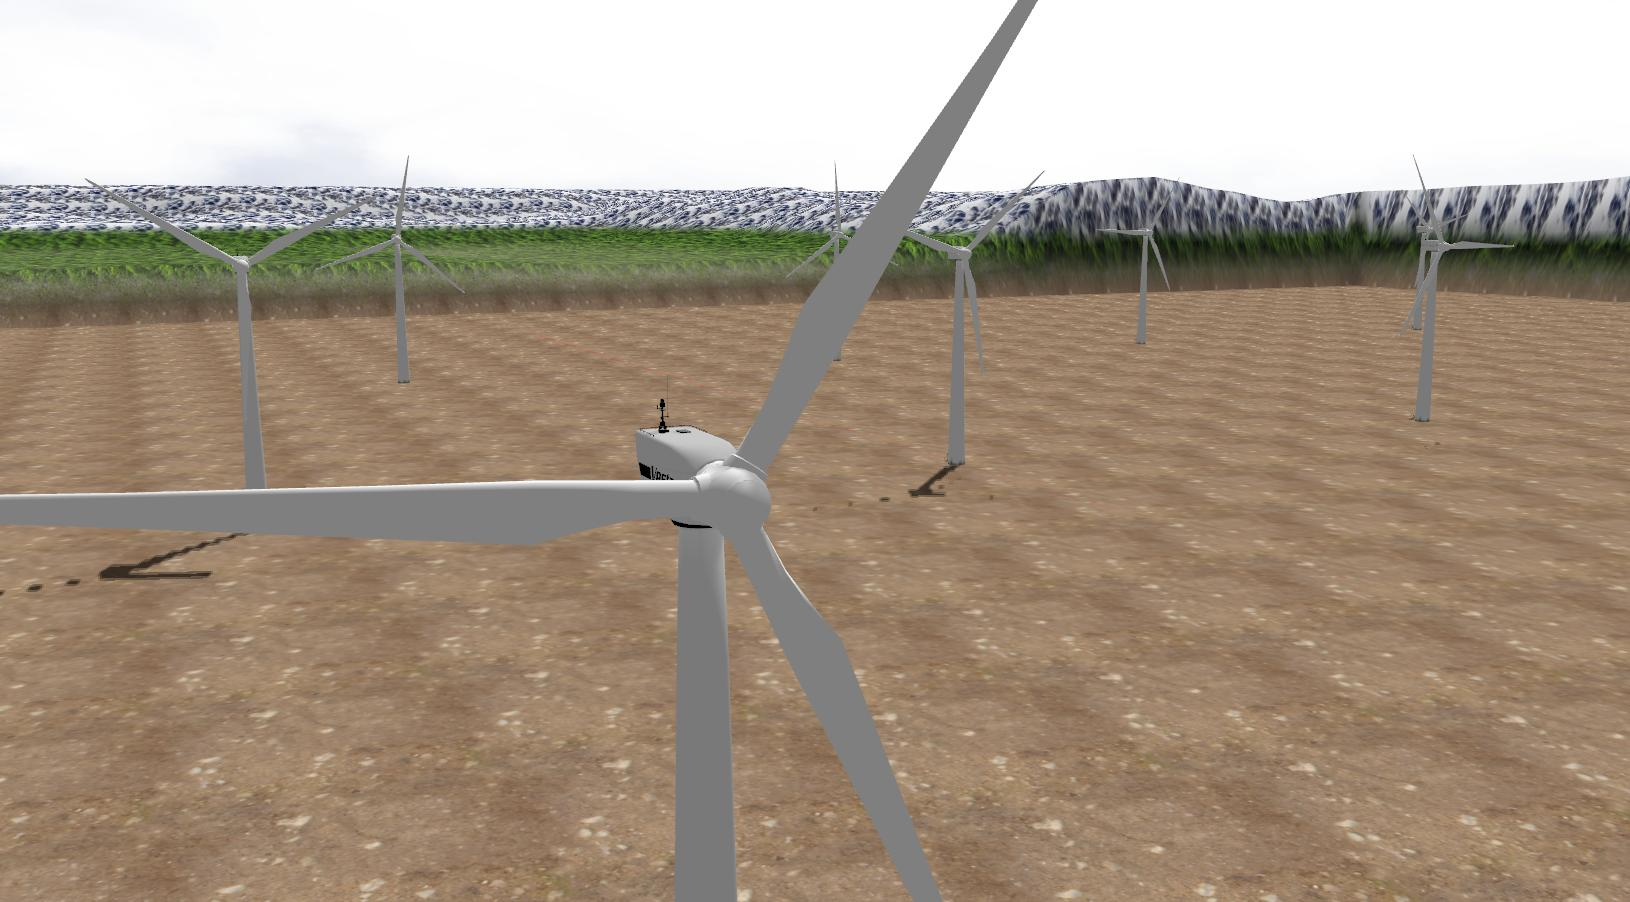
\includegraphics[width=\linewidth]{images/sim_vestas_multiple.jpg}
    (B)
  \end{minipage}
  \caption{Environnements de simulation.}
  \label{fig:sim_worlds}
\end{figure}

\subsubsection{Résultats par traitement d'images}

Tout d'abord, nous testons en simulation la méthode de Stokkeland modifiée. Nous pouvons observer dans la Figure \ref{fig:sim_detection} (A) une détection réussie en présence d'un angle de roulis et dans la Figure \ref{fig:sim_detection} (B) une détection lorsque l'horizon est présent près du rotor. Le grand cercle vert représente le rayon de recherche dans lequel les segments de pale sont recherchés, les petits cercles verts sont les intersections des projections des pales, le cercle rouge est la moyenne des intersections (le centre du rotor) et le cercle rose est la sortie du filtre de Kalman.
\begin{figure}[htbp]
  \centering
  \begin{minipage}{0.49\textwidth}
    \centering
    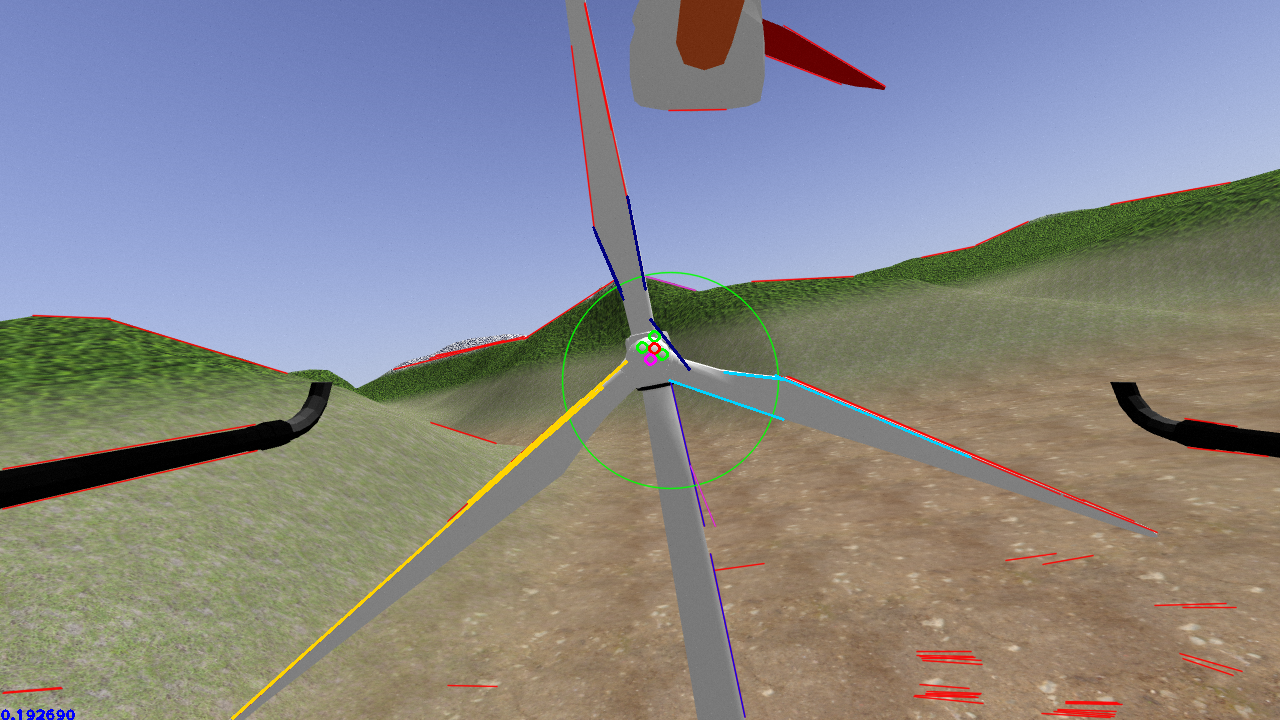
\includegraphics[width=\linewidth]{images/sim_detection.png} (A)
  \end{minipage}
  \begin{minipage}{0.49\textwidth}
    \centering
    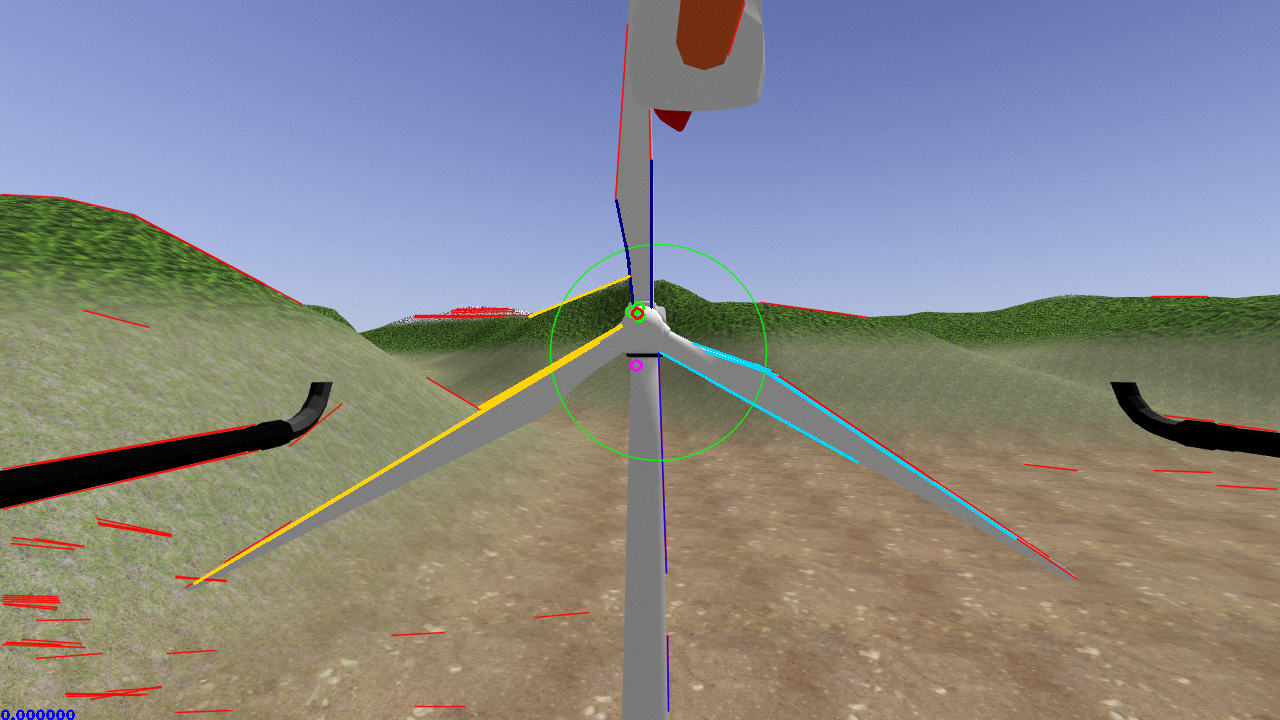
\includegraphics[width=\linewidth]{images/sim_detection3.png} (B)
  \end{minipage}
  \caption{Détections réussies en simulation.}
  \label{fig:sim_detection}
\end{figure}

Suite à plusieurs expérimentations, il devient difficile d'apprécier cette méthode et nous démontrons qu'une approche entièrement visuelle sans information au préalable n'est pas pratique. Dans nos tests, en simulant une trajectoire d'avance manuellement à l'aide d'une manette, le taux de détection varie grandement entre 10\% et 60\%, et dépend fortement du réglage des divers paramètres des filtres gaussiens, de la détection des contours et des lignes et des divers paramètres de distance de recherche. De plus, une fois les paramètres réglés pour augmenter le taux de détection, ceux-ci deviennent invalides lorsque l'on modifie les paramètres de l'environnement de simulation tels que l'angle des pales, la texture du sol, les nuages dans le ciel et la position de la source de lumière. Un autre problème rencontré est la difficulté de choisir les paramètres du flou gaussien tel que la texture de l'arrière-plan soit atténuée tout en préservant les contours de l'éolienne pour l'algorithme de Canny. En somme, il est impossible de régler les paramètres au préalable pour accommoder toutes les conditions possibles qui seront rencontrées sur le terrain.

Nous profitons de la présence de la caméra stéréo ZED simulée pour tester le fonctionnement de la résolution de la profondeur sur la surface de l'éolienne. Nous pouvons observer dans la Figure \ref{fig:stereo_fail} que la surface blanche de l'éolienne ne comporte pas assez de texture pour bien calculer la résolution stéréo. Résultat inattendu, le calcul de profondeur fonctionne parfois près de la bordure de l'objet où la transition entre la pale blanche et l'arrière-plan donne une caractéristique pouvant être mise en correspondance dans l'image de droite. Par contre, lorsque la pale est horizontale, elle devient quasi-invisible du fait que la bordure est parallèle à la géométrie épipolaire. Ce problème est bien connu par les chercheurs utilisant la vision stéréoscopique pour le calcul de profondeur. Certains tel que \citep{meier2017real} ont récemment proposé une solution possible à l'aide de caméras stéréo orthogonales; cependant la résolution de ce problème sort du cadre de ce projet.

\begin{figure}[htb]
  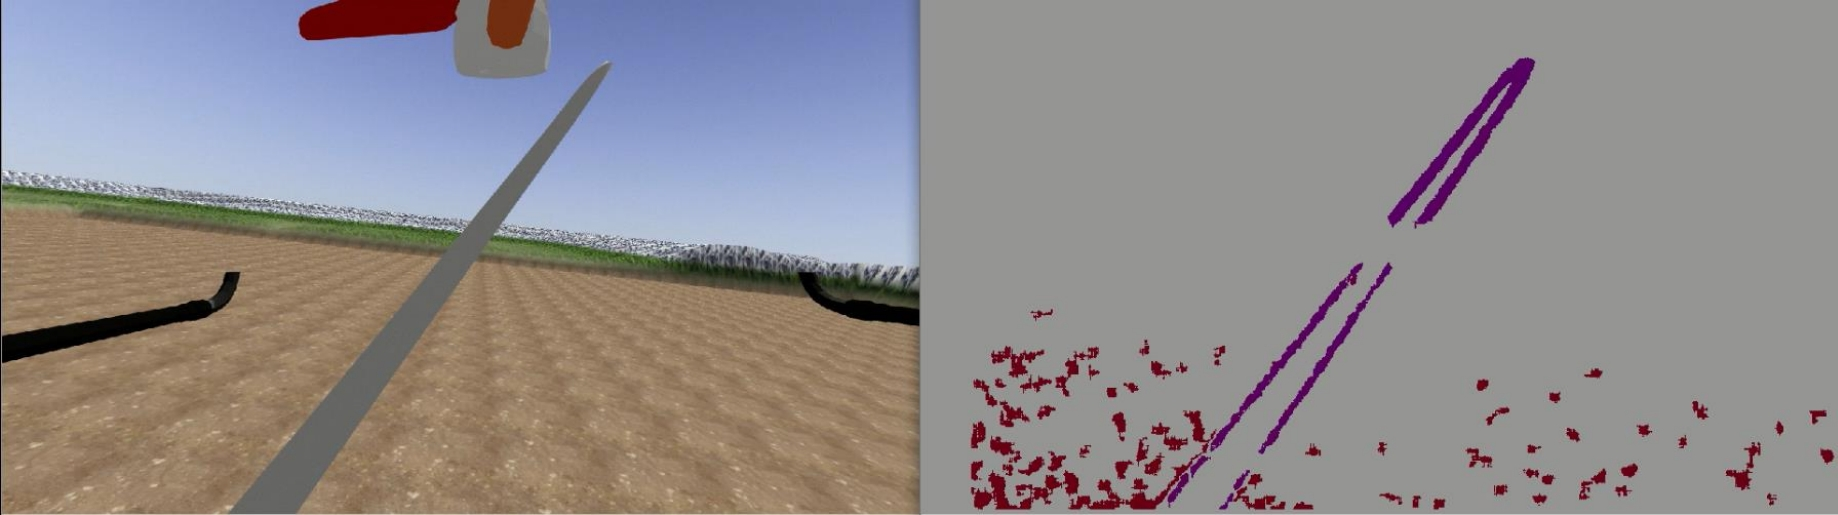
\includegraphics[width=\linewidth]{images/stereo_failure.jpg}
  \caption{Échec de la résolution de profondeur par correspondance de blocs.}
  \label{fig:stereo_fail}
\end{figure}

\subsubsection{Résultats du suivi par laser}

La mission d'inspection entièrement par laser se déroule avec succès dans une grande variété de scénarios. Dans cette section, nous présentons et analysons l'un des vols effectués sur une éolienne avec pour seule information \textit{a priori} que l'une des pales a été placée vers le haut. Dans la Figure \ref{fig:sim_tower_total}, on peut observer la trajectoire entière exécutée par l'UAV avec les différentes phases séparées par couleur. Outre une petite discontinuité dans la trajectoire de la troisième pale, la majorité du vol s'exécute de façon continue.
\begin{figure}[!htb]
  \centering
  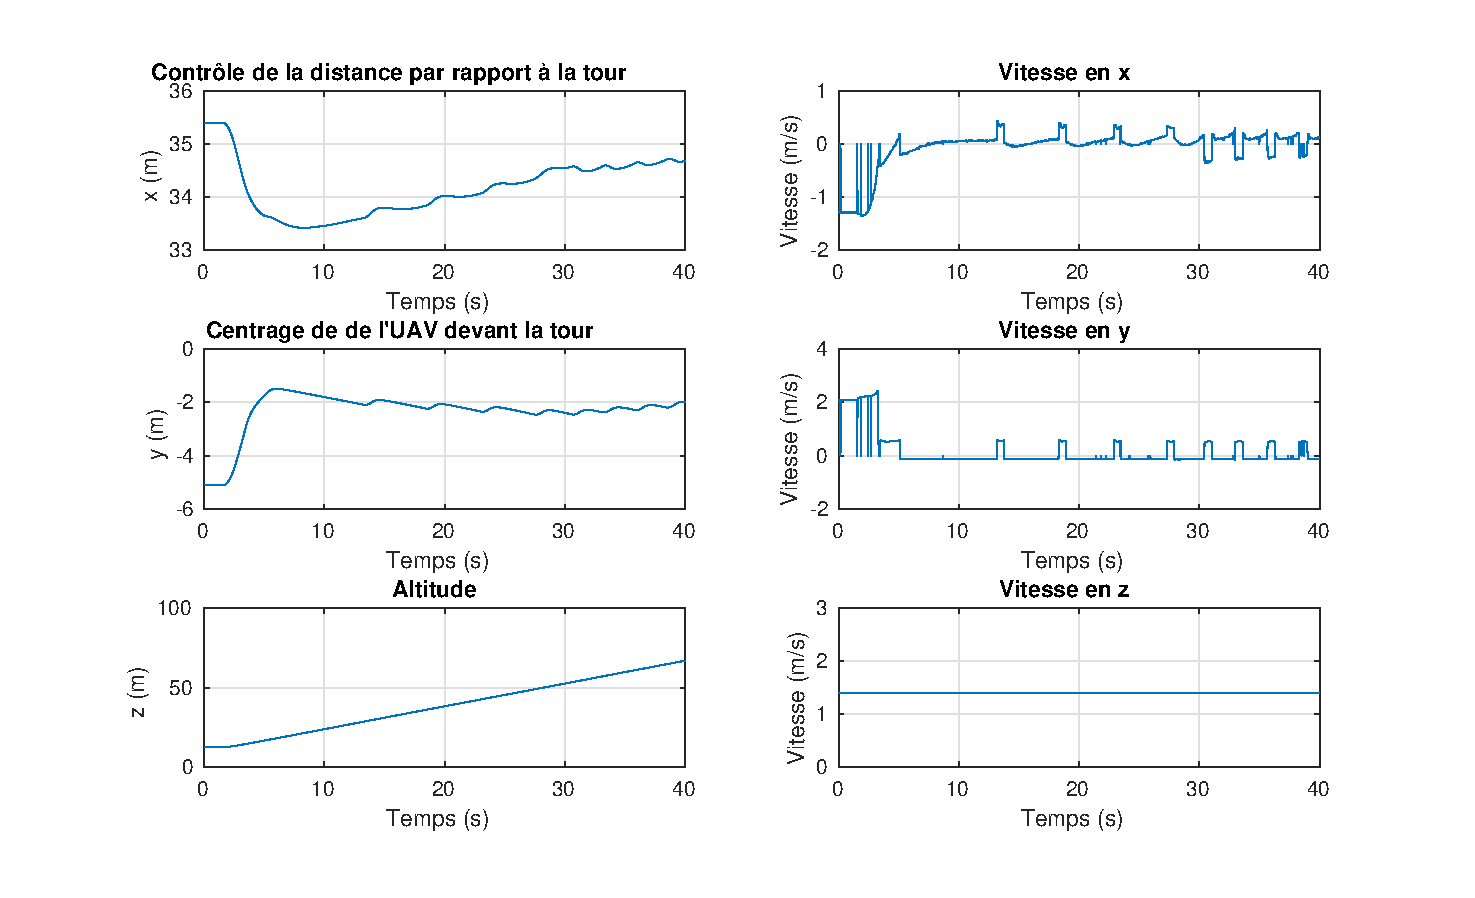
\includegraphics[width=\linewidth]{images/sim_tower_ascent}
  \caption{Trajectoire suivie pour la montée de la tour et les commandes de vitesse associées.}
  \label{fig:sim_tower_ascent}
\end{figure}

Dans la Figure \ref{fig:sim_tower_ascent}, nous pouvons voir la décomposition de la trajectoire suivie pour monter la tour. L'UAV commence légèrement décentré par rapport à la tour et tente immédiatement de se centrer. La vitesse commandée en $z$ est constante et on voit que l'altitude augmente de façon constante. Par contre, on peut voir que les déplacements en $x$ et en $y$ sont légèrement saccadés. En $x$, la raison est une combinaison de gains PID légèrement trop agressifs et du fait que le diamètre de la tour change au fur et à mesure qu'elle monte. En $y$, le problème provient plutôt de la faible résolution du scanner laser. Avec seulement $8$ points, la bordure de la tour se retrouve entre deux rayons du laser. Les différentes bosses dans la courbe $v_y$ correspondent aux instants où l'un des rayons adjacents au centre frappe la tour. À cet instant le terme d'erreur devient non nul et le robot bouge latéralement.
\begin{figure}[htb]
  \centering
  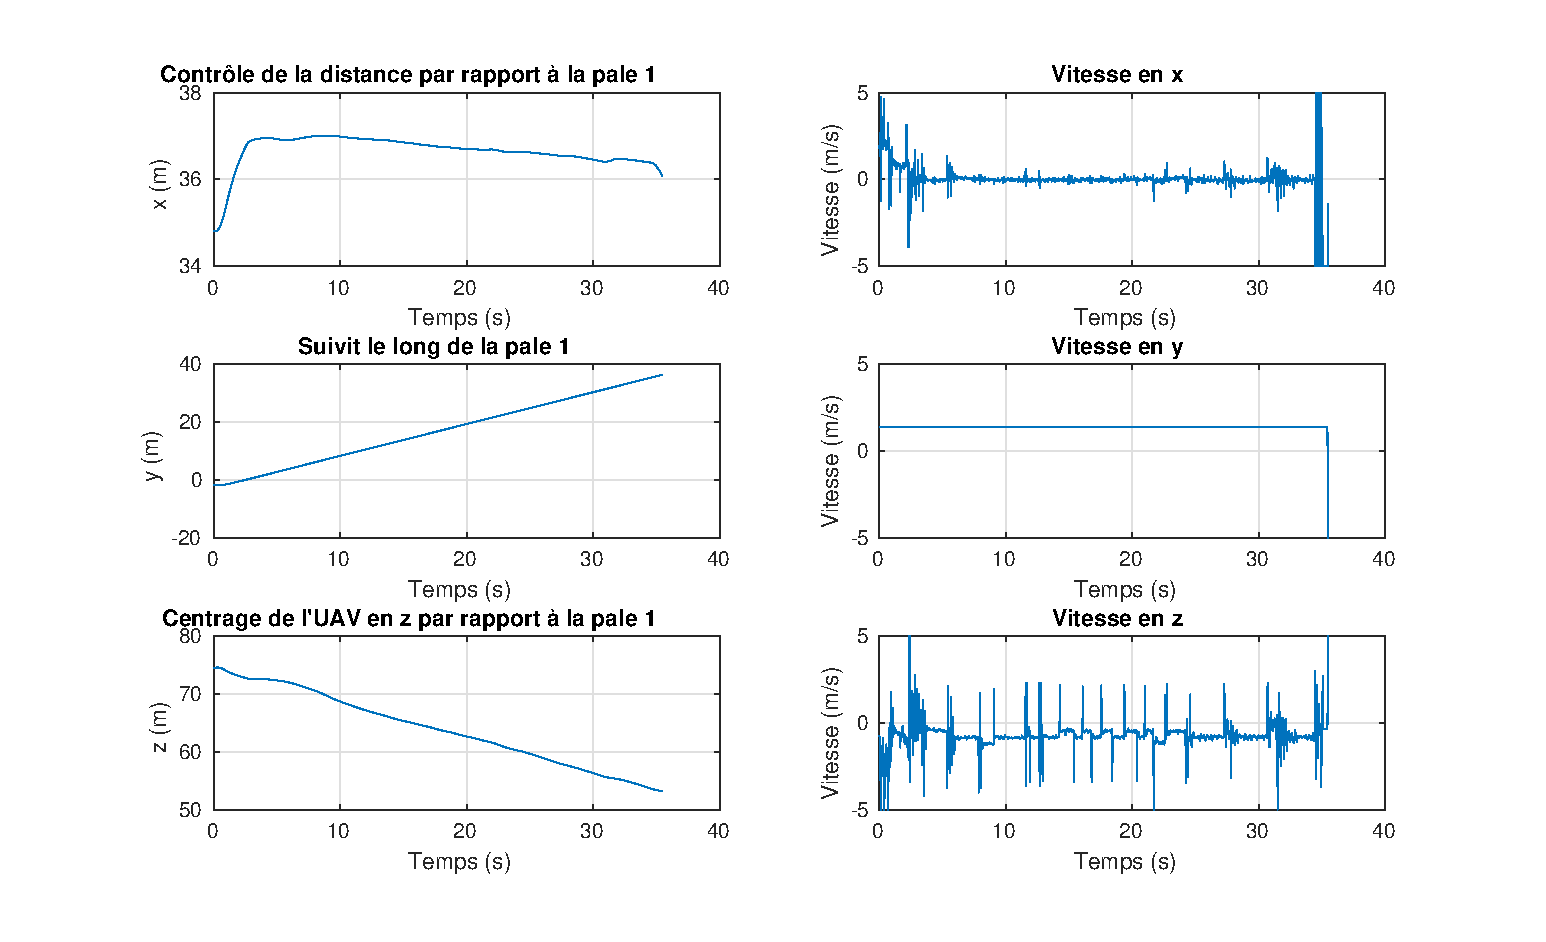
\includegraphics[trim=30 20 30 0, clip, width=\linewidth]{images/sim_suivit_pale}
  \caption{Trajectoire pour le suivi de la pale 1.}
  \label{fig:sim_suivit_pale}
\end{figure}

La Figure \ref{fig:sim_suivit_pale} présente la trajectoire et les commandes de vitesses pour le suivi de la pale 1. Nous voyons que les vitesses en $z$ semblent saccadées, mais ceci est encore dû au petit nombre de rayons du scanner laser. Chaque petit pic est en fait un instant où un rayon supplémentaire du laser parvient à toucher la surface de la pale et influencer le calcul de son centre. Vers la fin de la courbe, $v_x$ nous pouvons observer une oscillation entre les commandes $0$, $+5$ et $-5$ mètres par seconde. Ceci est dû au fait que le bout de la pale est assez petit pour passer entre deux rayons du scanner laser, combiné au mouvement de tangage du véhicule pour avancer et reculer, le laser parvient momentanément à toucher la pale. En réalité ceci ne devrait pas être un problème, car le LeddarVu8 ne souffre pas des angles morts entre ses rayons. Malgré cela, le robot poursuit son chemin jusqu'à ce que le bout de la pale soit officiellement détectée par le compteur de lectures vides.
\begin{figure}[htb]
  \centering
  \includegraphics[trim=30 10 10 50,clip,width=0.5\linewidth]{images/sim_tower_total}
  \caption{Trajectoire complète d'inspection.}
  \label{fig:sim_tower_total}
\end{figure}

\clearpage
\subsection{Résultats de tests sur le terrain}
\label{subsec:results_field}

\begin{figure}[htb]
  \centering
  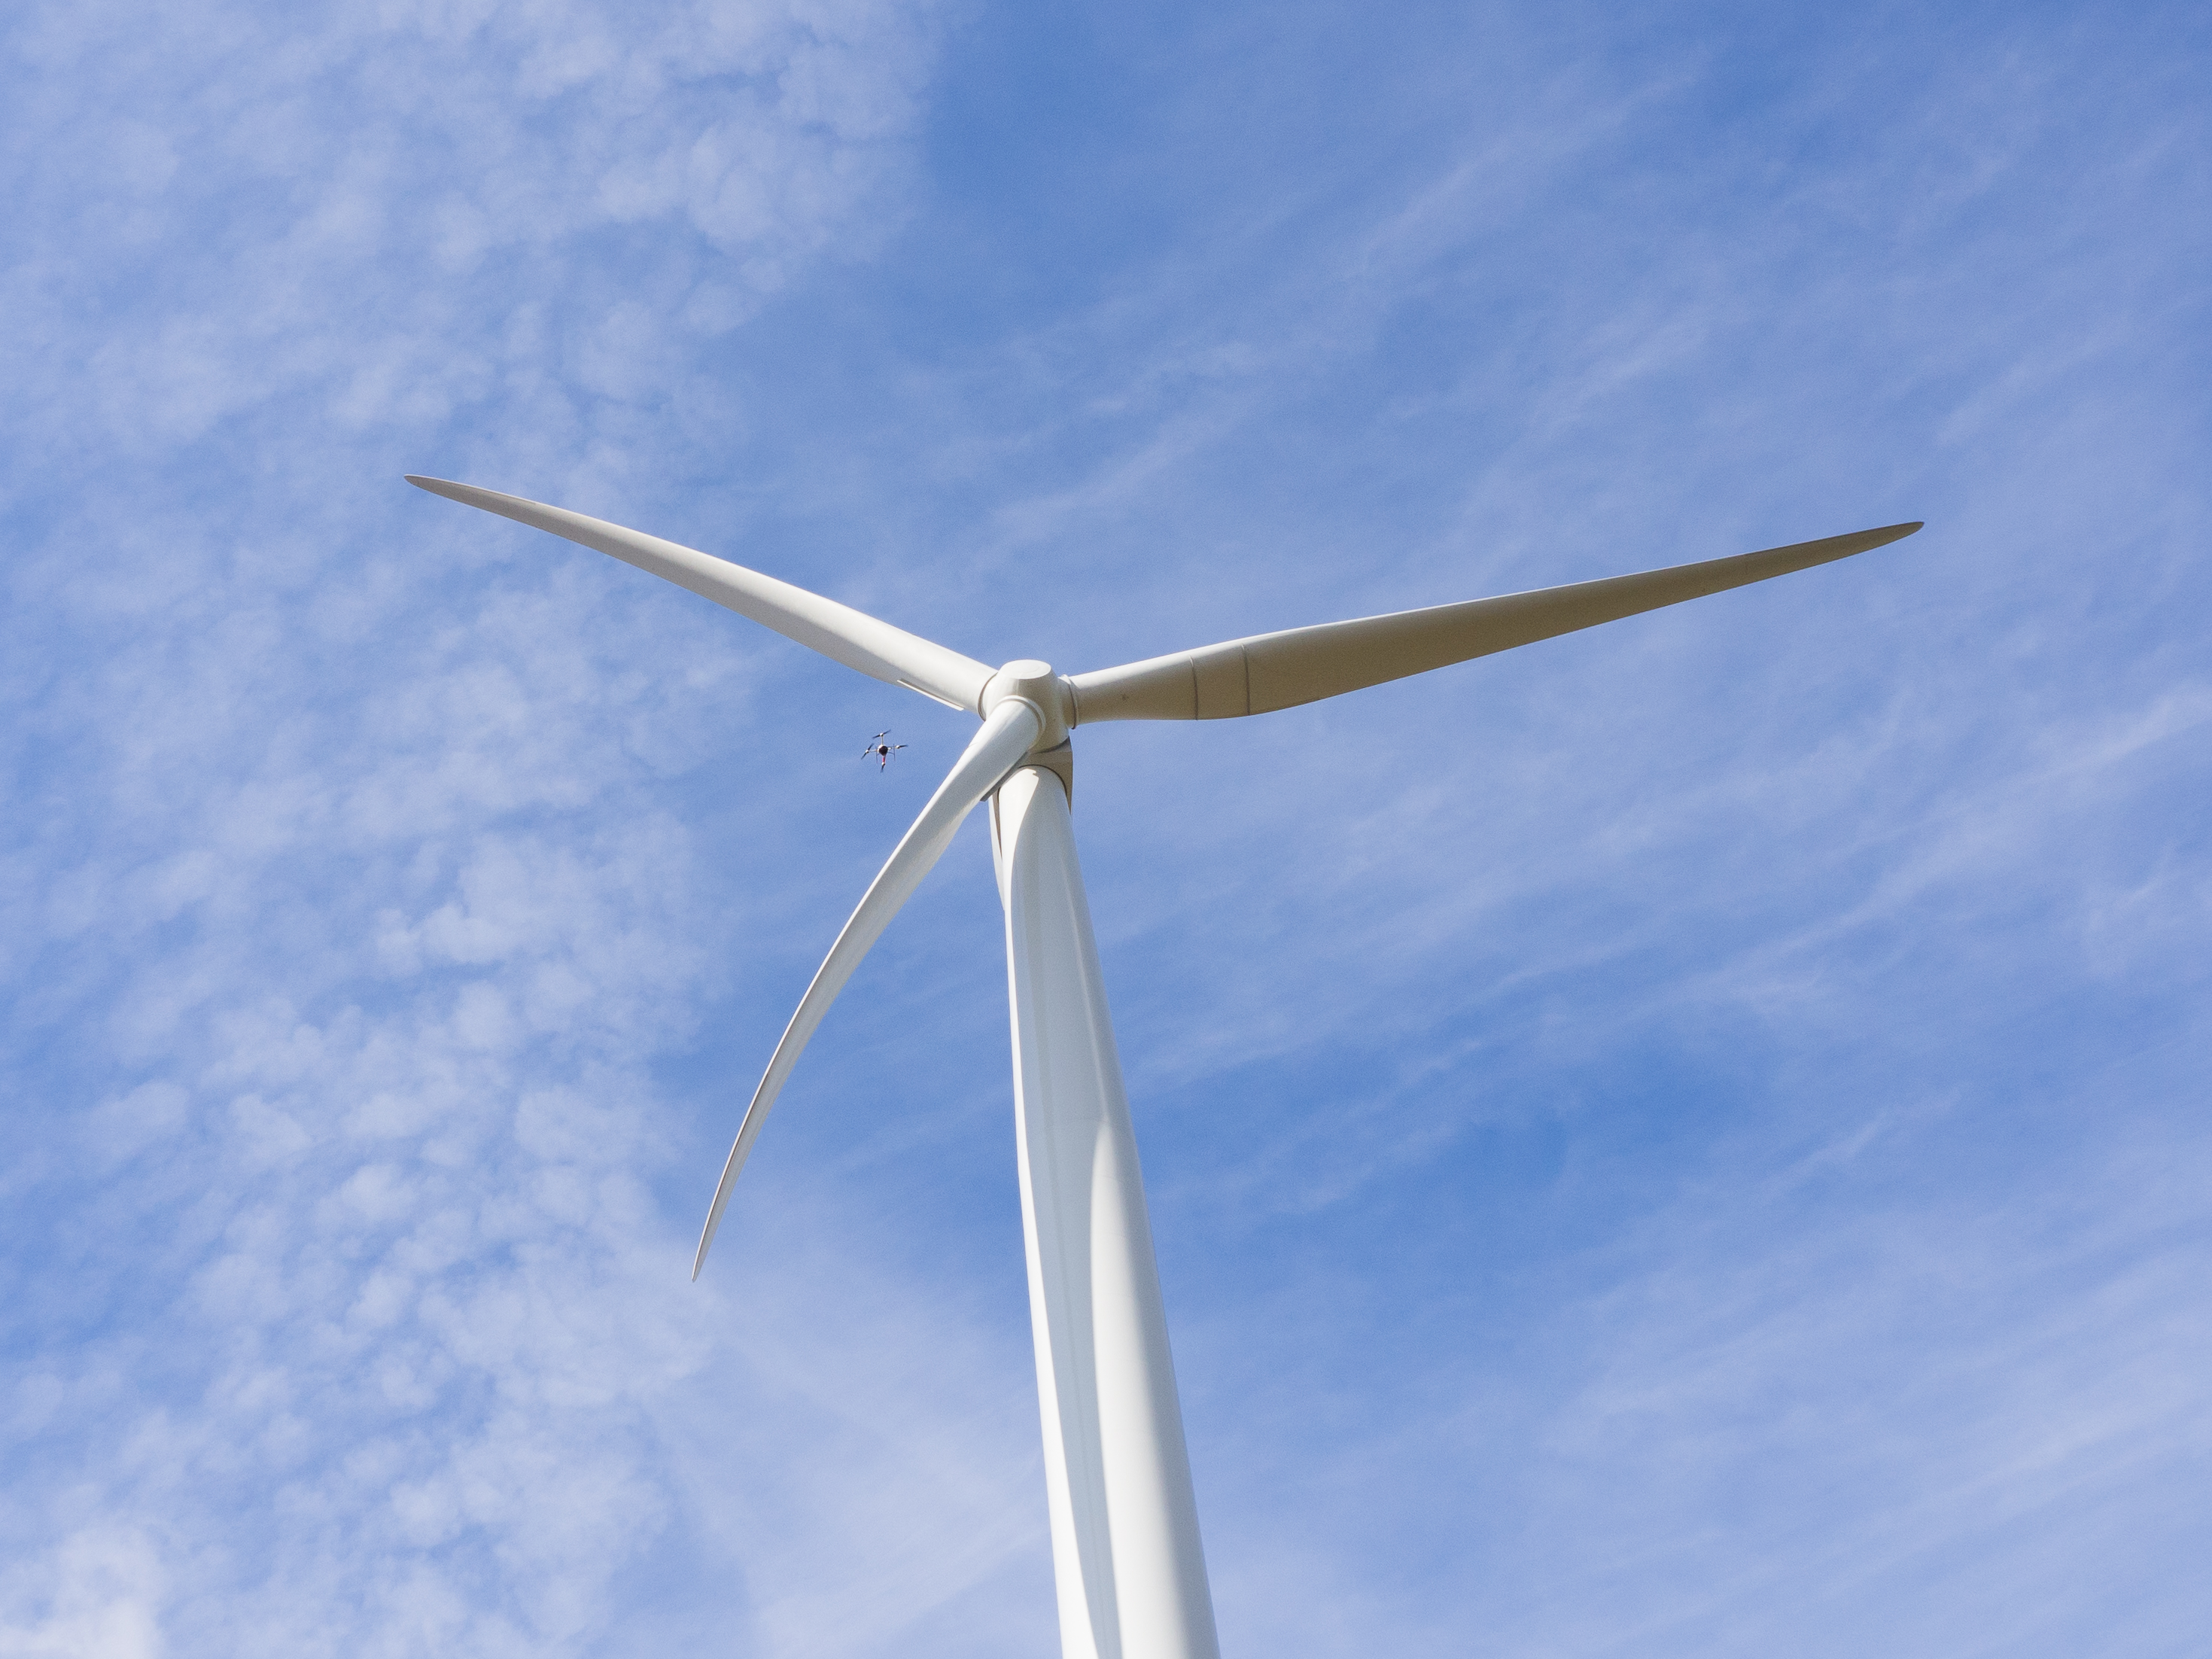
\includegraphics[trim=180 200 180 180,clip,width=\linewidth]{images/test_eolienne.jpg}
  \caption{Le md4-1000 en vol inspectant l'une des pales.}
  \label{fig:test_eolienne}
\end{figure}

Suivant les spécifications initiales, l'intégration des capteurs s'est faite sur un md4-1000 pris en photo dans la Figure \ref{fig:field_vehicle} pour faire un test de vol manuel nous permettant de confirmer certaines de nos hypothèses au niveau de la vision stéréo. Le système d'exploitation Ubuntu 16.04 a été installé sur l'ordinateur Nvidia TX2 avec des modifications apportées au noyau Linux fourni par Nvidia afin de permettre au TX2 de s'interfacer avec les différents périphériques montés sur la carte mère AuvIdea J140. Les LeddarVu8 et la caméra ZED sont branchés par USB3 alors que la communication au md4-1000 se fait par UART.

\begin{figure}[htp]
  \centering
  \begin{minipage}{0.45\textwidth}
    \centering
    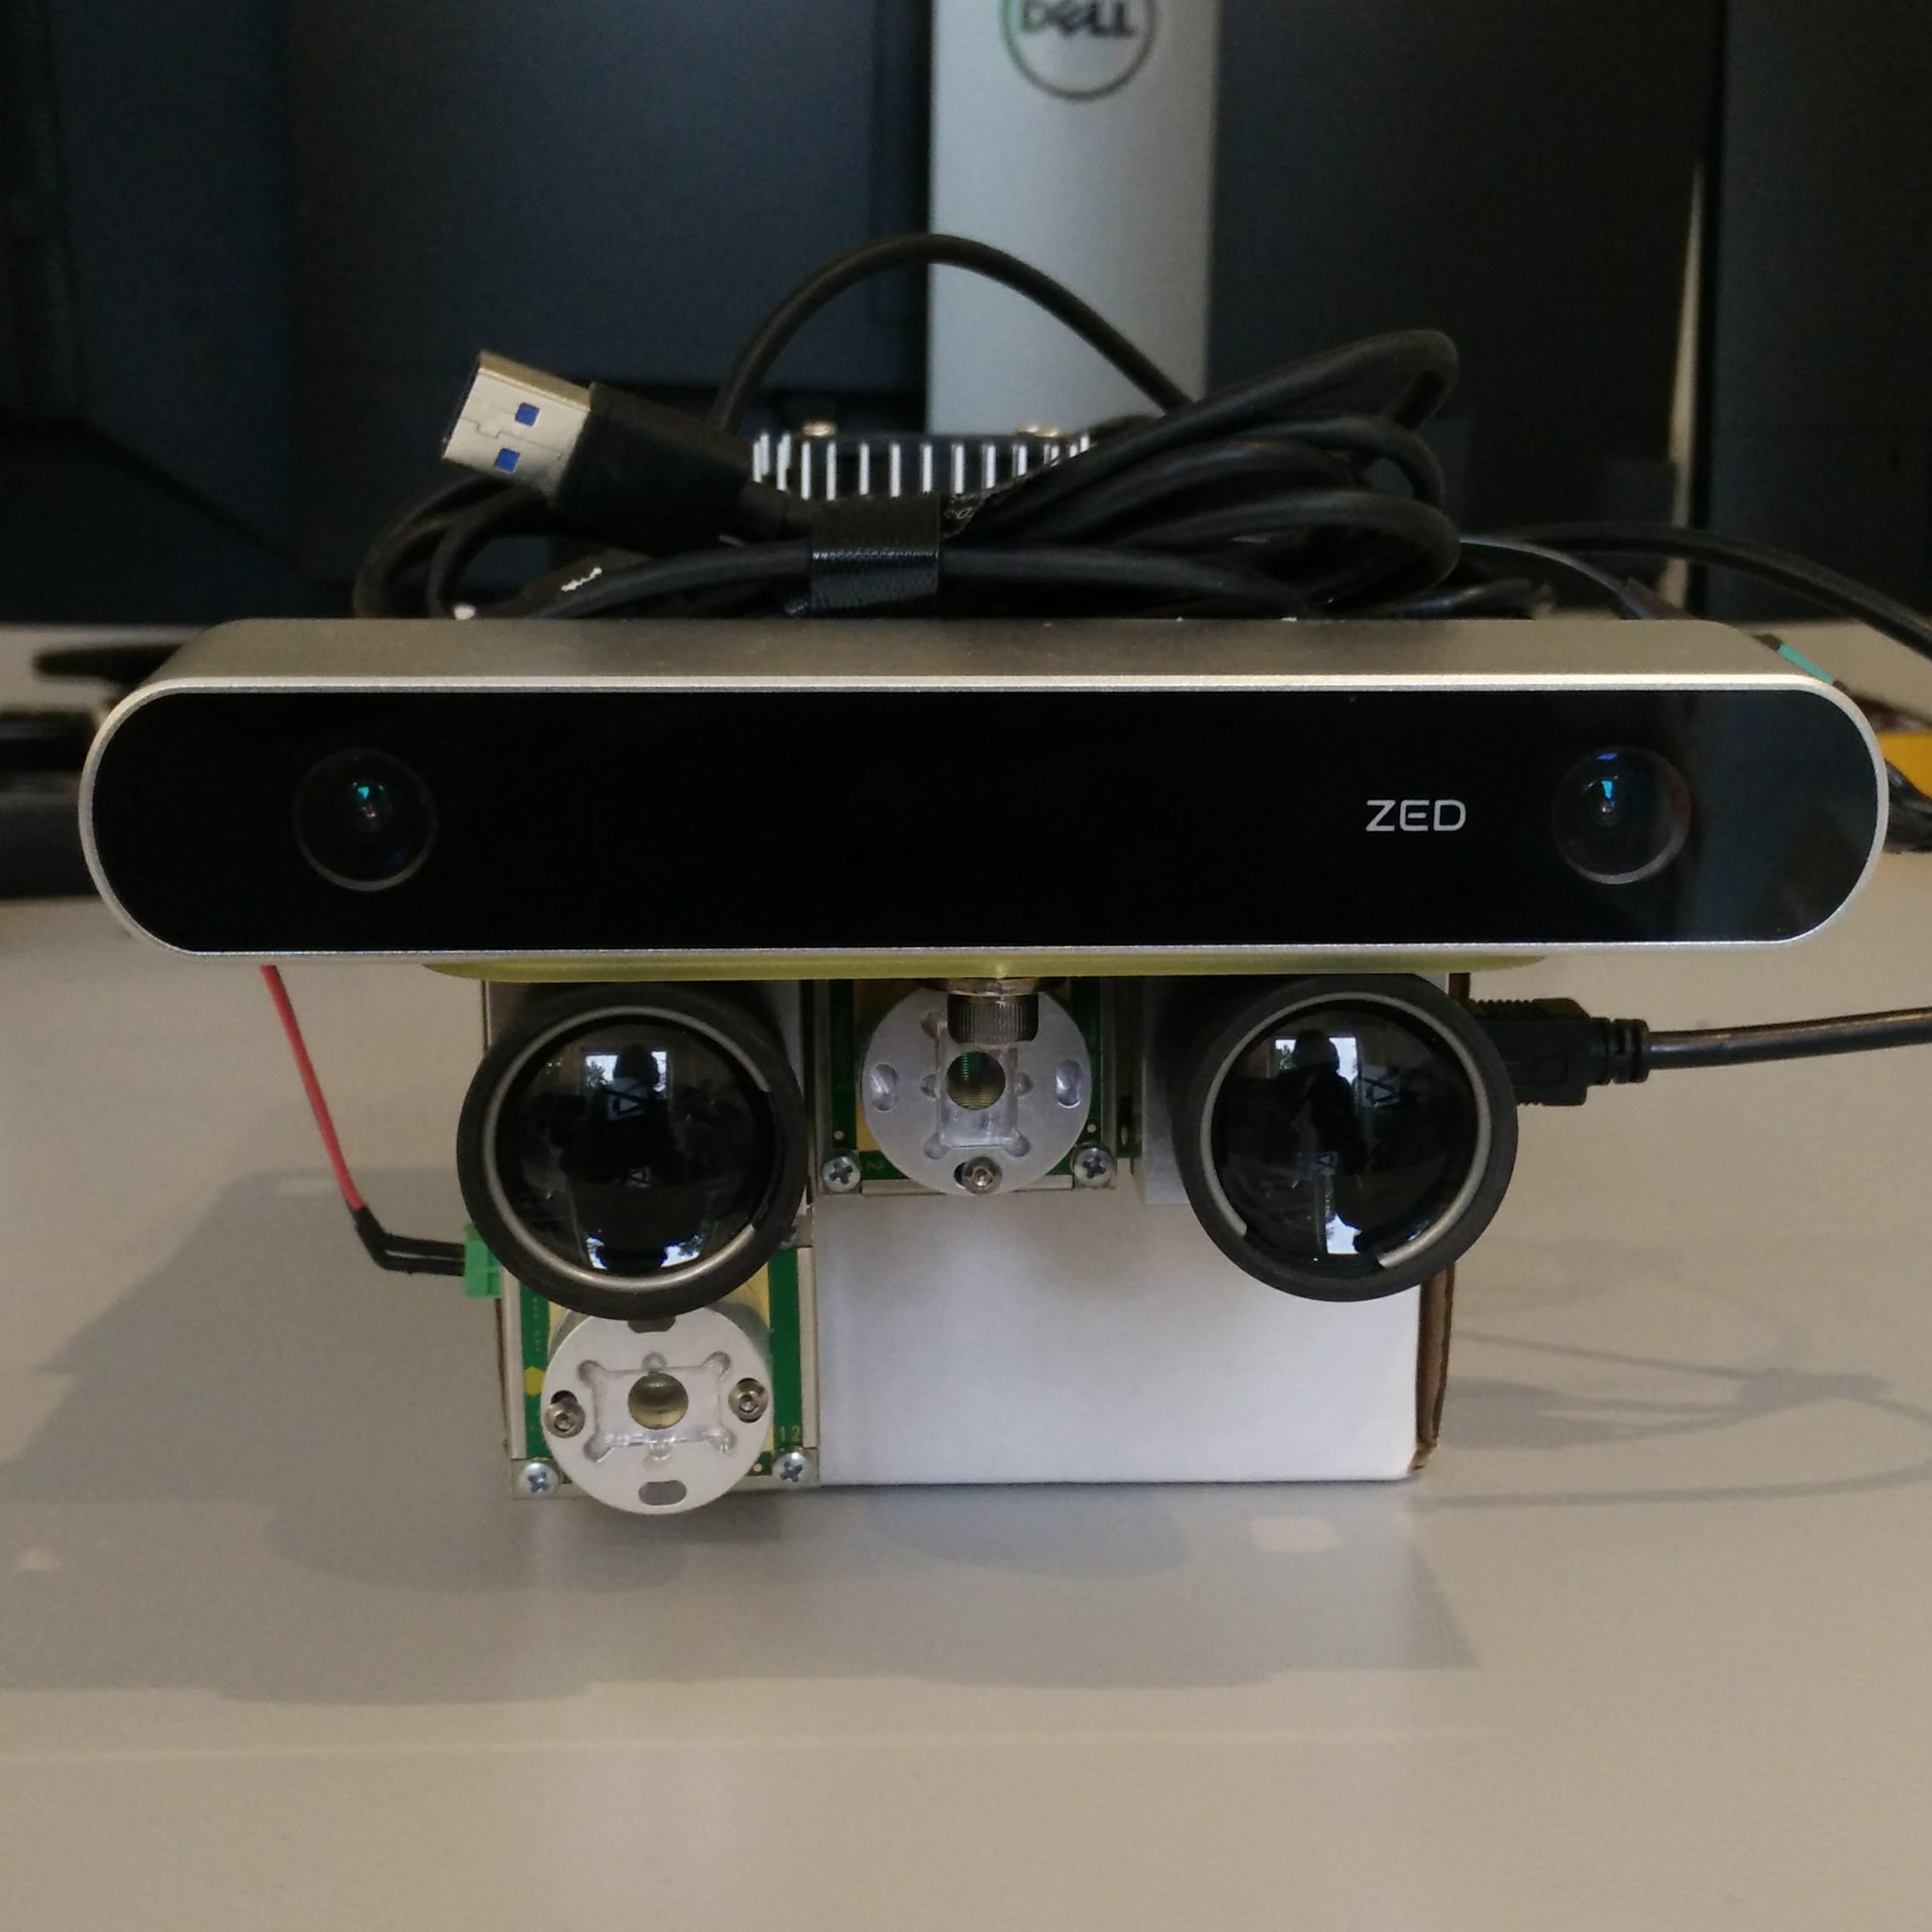
\includegraphics[width=\linewidth]{images/payload.jpg}
    (A)
  \end{minipage}
  \begin{minipage}{0.45\textwidth}
    \centering
    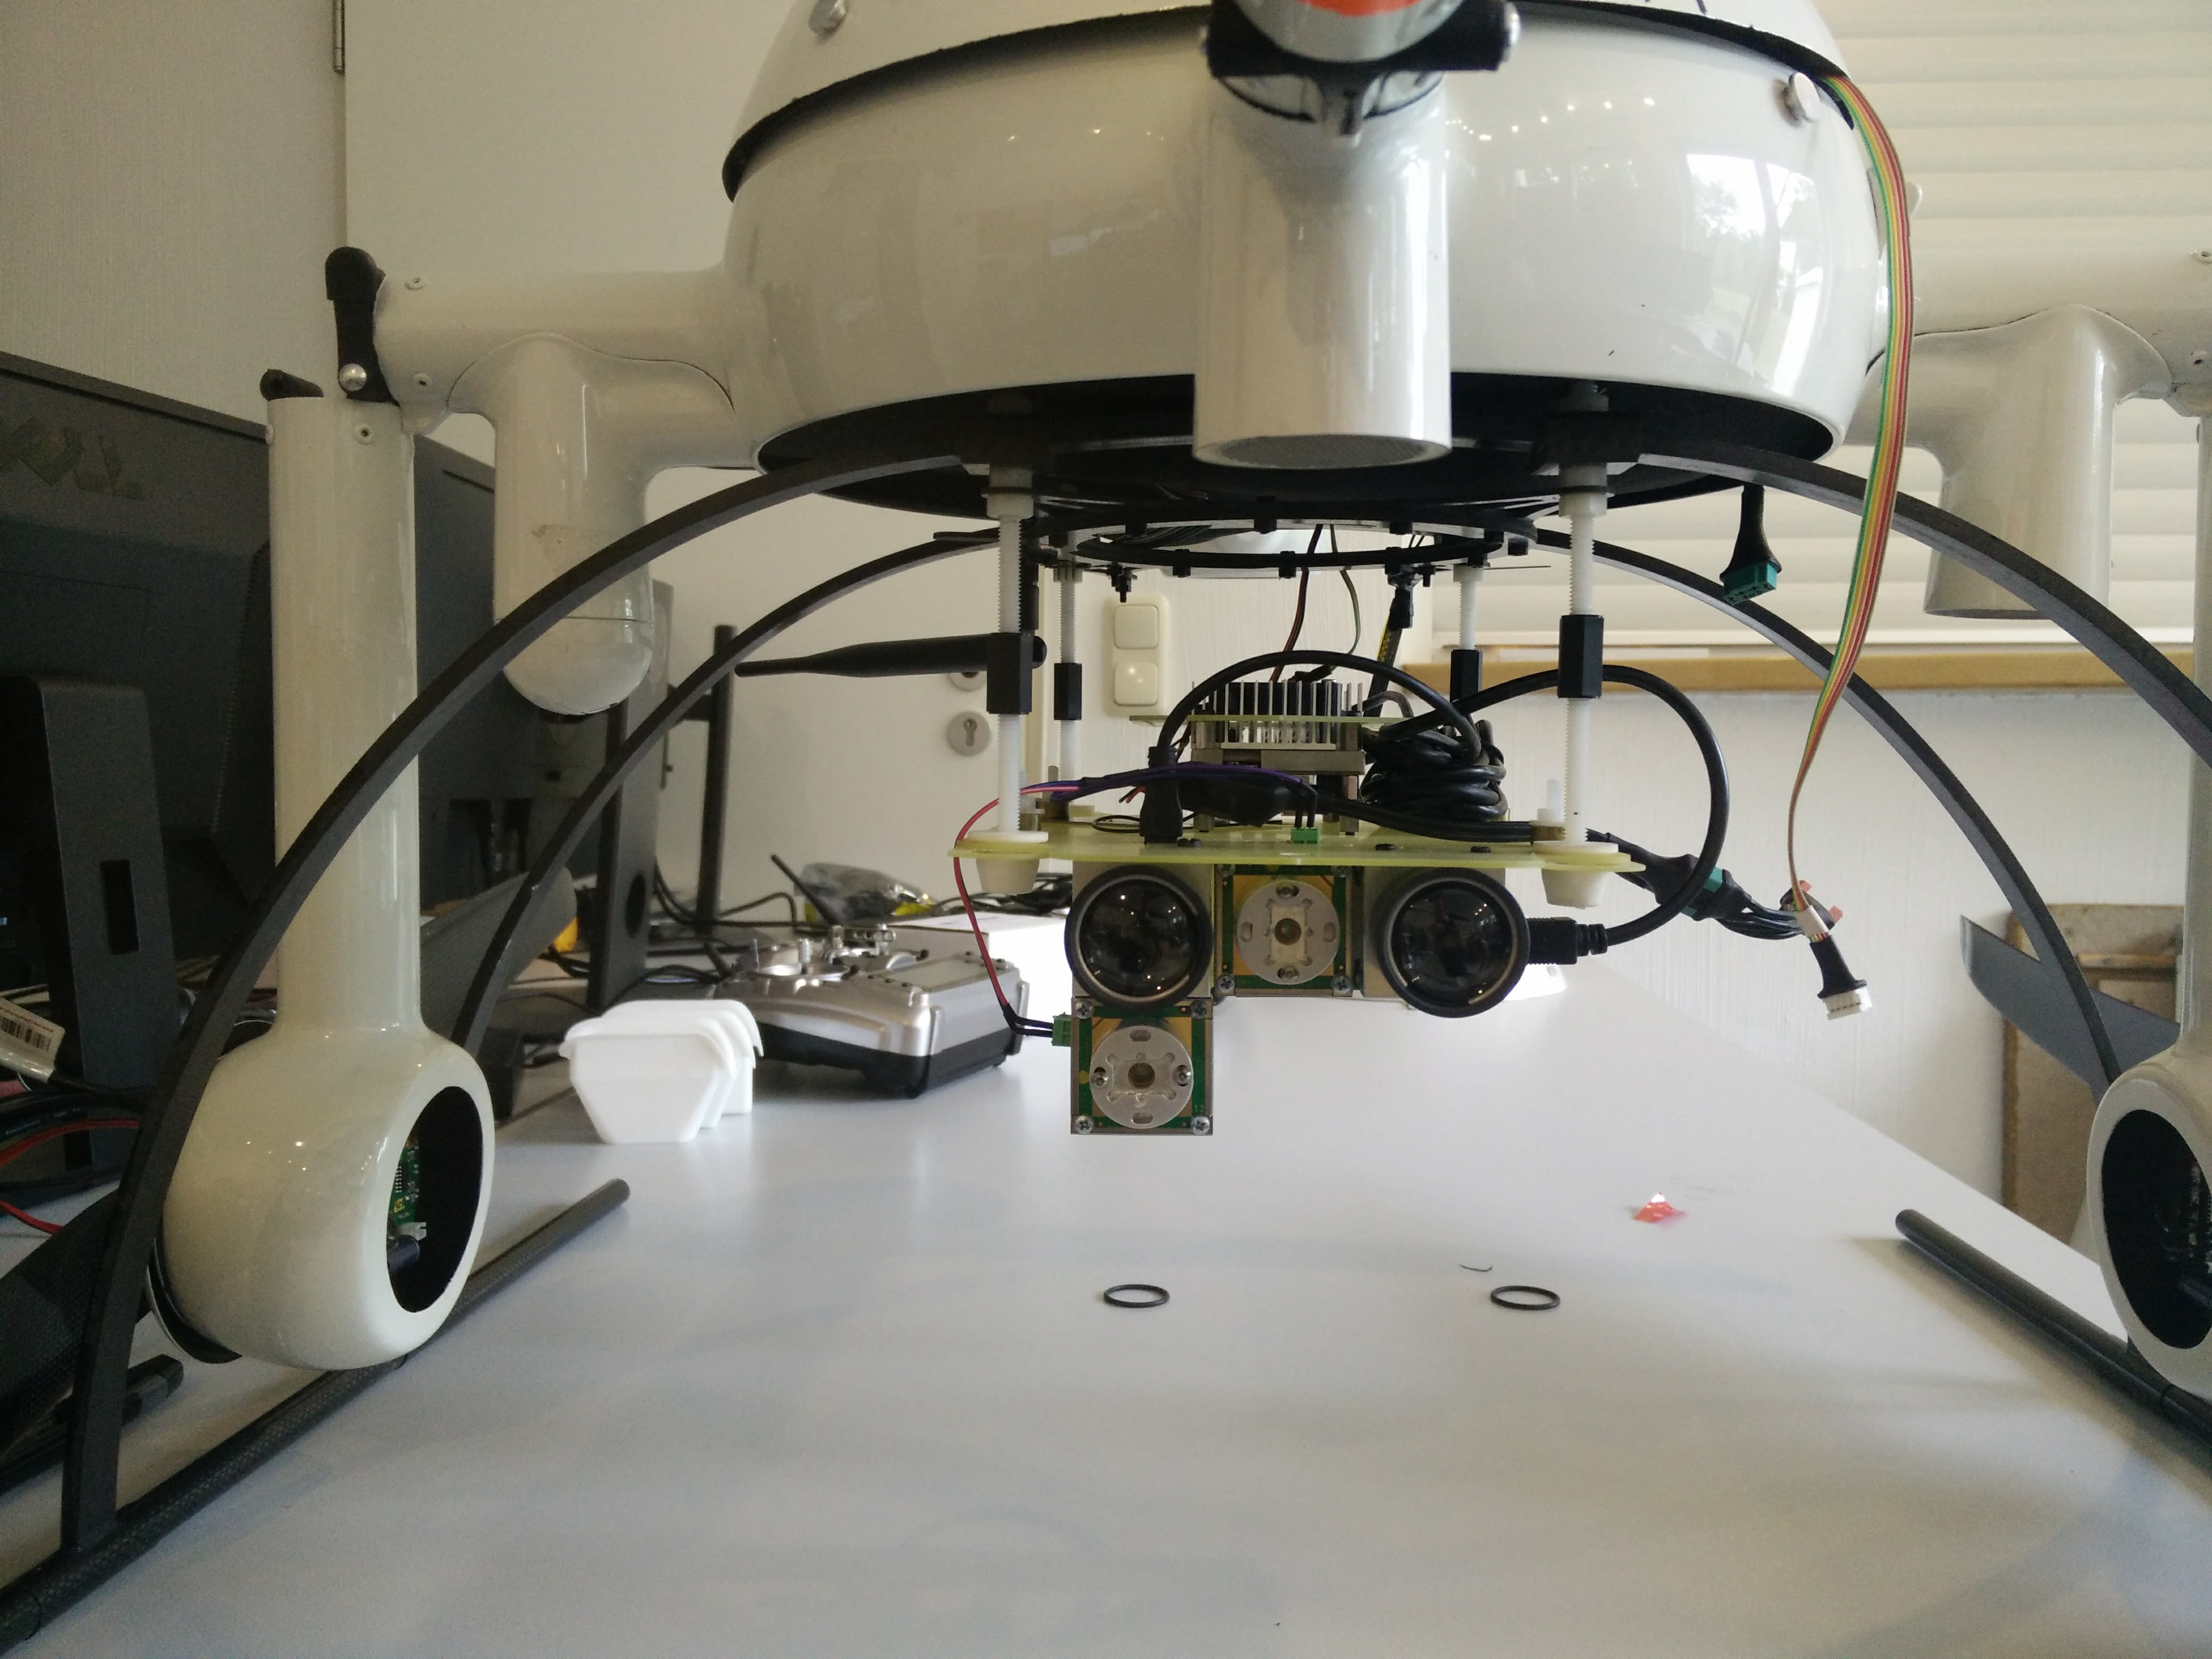
\includegraphics[width=\linewidth]{images/payload2.jpg}
    (B)
  \end{minipage}
  \caption[Véhicule md4-1000 avec les capteurs et l'ordinateur de bord intégrés]{Véhicule md4-1000 avec les capteurs et l'ordinateur de bord intégrés. (A) Caméra ZED et les télémètres lasers LeddarVu8. (B) La charge utile installée sur le robot (sans la ZED), avec la Nvidia TX2 visible.}
  \label{fig:field_vehicle}
\end{figure}

Les tests de vol ont été effectués au parc éolien Pierre-de-Saurel où la hauteur de la tour est de $100$ mètres et le diamètre du rotor incluant les pales est de $92.5$ mètres. La Figure \ref{fig:test_eolienne} nous donne un ordre de grandeur de la structure par rapport à l'UAV.

% En collaboration avec le personnel de Microdrones, une procédure d'inspection a été développée pour assurer une mission sécuritaire.
%
% \begin{enumerate}
%   \item La nacelle est tournée en aval du vent, c'est-à-dire que le vent arrive de l'arrière de l'éolienne. Ceci a pour effet que si jamais le signal GPS est perdu ou que l'interférence magnétique cause une perte du contrôle de position, l'UAV s'éloignera de la structure.
%   \item Les pales sont tournées parallèles au vent pour les empêcher de tourner.
%   \item Un système de télémétrie relai au pilote la distance moyenne des objets détectés par les lasers.
%   \item Un observateur se place près de la tour pour prévenir le pilote de dangers de collision.
% \end{enumerate}

La caméra stéréo s'avère à avoir une performance extrêmement variable à travers le vol tel qu'on peut le voir dans la Figure \ref{fig:field_stereo_fail}. Il est difficile de corréler exactement les caractéristiques de la scène au succès ou à l'échec de la résolution de profondeur. Dans certains cas, une pale diagonale est invisible alors que dans le dernier exemple, elle est parfaitement visible. On voit aussi que le ciel clair est parfois résolu par erreur. Par conséquent, nous prouvons notre hypothèse initiale et en concluons qu'une caméra stéréo est inutilisable dans le contexte de l'inspection d'éoliennes.

\begin{figure}
  \begin{tabular}{cc}
    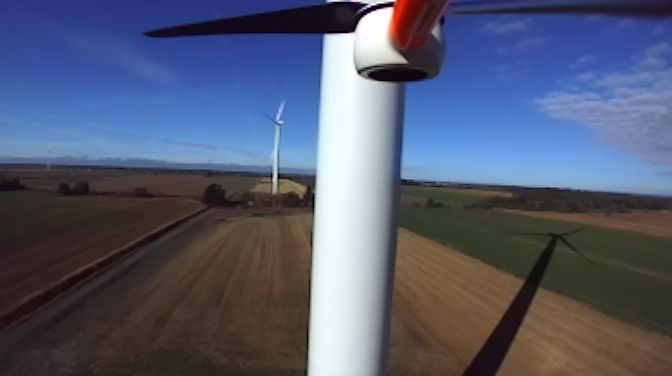
\includegraphics[width=0.5\linewidth]{images/field_stereo_fail_rgb.png} &
    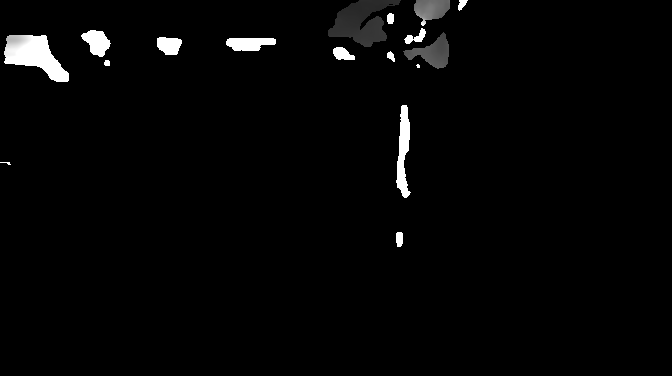
\includegraphics[width=0.5\linewidth]{images/field_stereo_fail_pcl.png} \\
    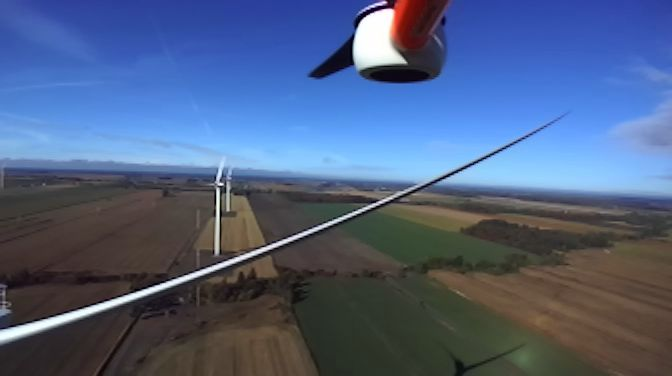
\includegraphics[width=0.5\linewidth]{images/field_stereo_fail_rgb2.png} &
    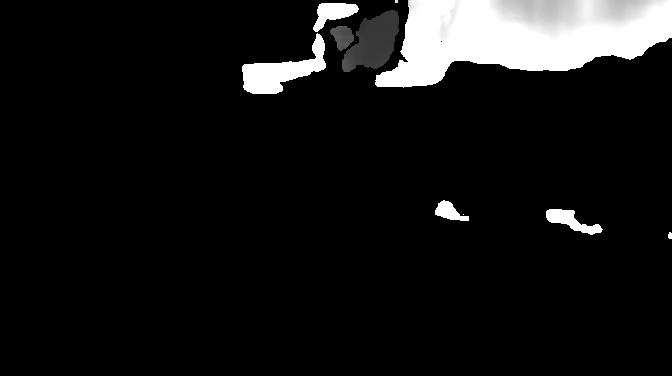
\includegraphics[width=0.5\linewidth]{images/field_stereo_fail_pcl2.png} \\
    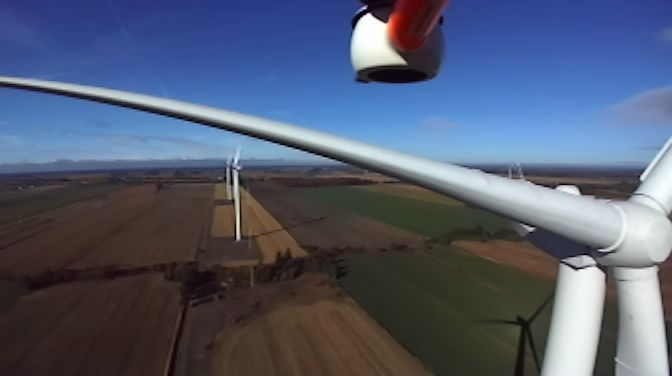
\includegraphics[width=0.5\linewidth]{images/field_stereo_success_rgb.png} &
    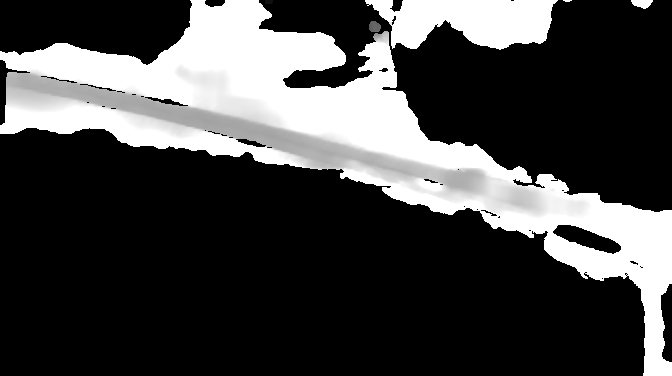
\includegraphics[width=0.5\linewidth]{images/field_stereo_success_pcl.png} \\
    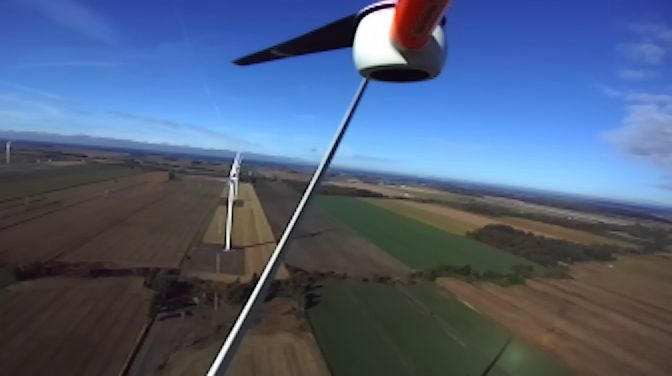
\includegraphics[width=0.5\linewidth]{images/field_stereo_success_rgb2.png} &
    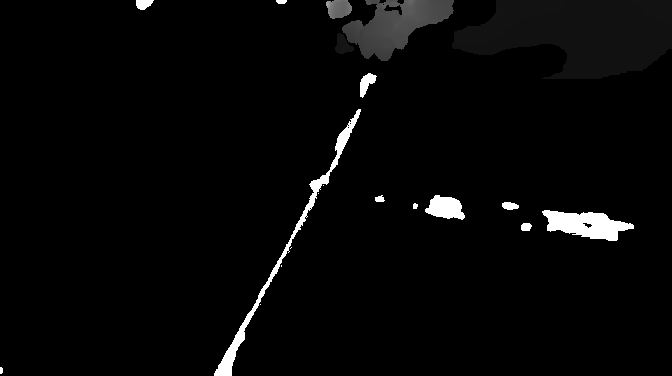
\includegraphics[width=0.5\linewidth]{images/field_stereo_success_pcl2.png} \\
  \end{tabular}
  \caption[Exemples de succès et d'échecs de perception de distance]{
  Exemples de succès et d'échecs de perception de distance. À gauche, les images RGB de la caméra de gauche, et à droite, les images de profondeur ramenées sur la caméra de gauche.}
  \label{fig:field_stereo_fail}
\end{figure}

En ce qui concerne l'approche par laser il n'a pas été possible de tester le système sur le terrain en raison de différentes circonstances et d'une erreur logicielle survenue le jour du test. Plus de temps serait requis pour faire l'intégration et le réglage des gains PID sur le vrai véhicule. Par contre, puisque l'entièreté du logiciel est déjà écrite en C++ et prête à installer sur le véhicule, il ne suffirait que de changer quelques branchements au niveau des flux de données pour faire les tests sur le terrain.

\clearpage
\section{Discussion des résultats et travaux futurs}
\label{uav:results_conclusion_future_work}

Bien que nous n'avons pas pu valider notre approche sur le terrain, les résultats en simulation demeurent prometteurs et l'inspection d'éoliennes reste un projet important à poursuivre dans le futur. Par contre, suite à nos tests de vol manuels sur le terrain, nous réalisons maintenant que la méthode d'inspection bénéficierait de plusieurs changements.

Tout d'abord, pour qu'un UAV entre $1$ et $25$ kg utilisé à des fins non récréatives soit exempt du besoin d'un Certificat d'Opération Aériennes Spécialisées (COAS) par Transport Canada, il doit demeurer en dessous d'une altitude de $300$ pieds ($91$ mètres) \citep{transportscanada2016}. Puisque les grandes éoliennes ont leur nacelle à une altitude de $100$ mètres ou plus, ceci impliquerait que chaque fois qu'un inspecteur voudrait aller travailler, il faudrait appliquer pour un COAS à l'avance, ce qui peut prendre beaucoup de temps à être approuvé. Sans quoi, l'UAV n'aurait pas le droit d'inspecter les pales autres que celles pointant vers le bas.

Il reste néanmoins une alternative possible qui comporterait plusieurs avantages sur le système proposé à condition de remettre en question les modalités de la participation de l'inspecteur et du budget alloué. Le système pourrait faire une inspection en 3 dimensions d'une seule pale à la fois pointée vers le bas suivant une trajectoire présentée dans la Figure \ref{fig:alternative}. En commençant sur le côté de la pale l'UAV longerait la pale vers bas. Il pivoterait ensuite pour remonter le bord d'attaque avant de pivoter une dernière fois pour longer le côté droit. Ceci demanderait des capteurs différents et nécessiterait que l'inspecteur fasse tourner les pales entre chaque vol. On aurait aussi l'avantage d'avoir de bien meilleures images puisque la caméra serait pointée perpendiculairement à la surface à inspecter.

\begin{figure}[htb]
  \centering
  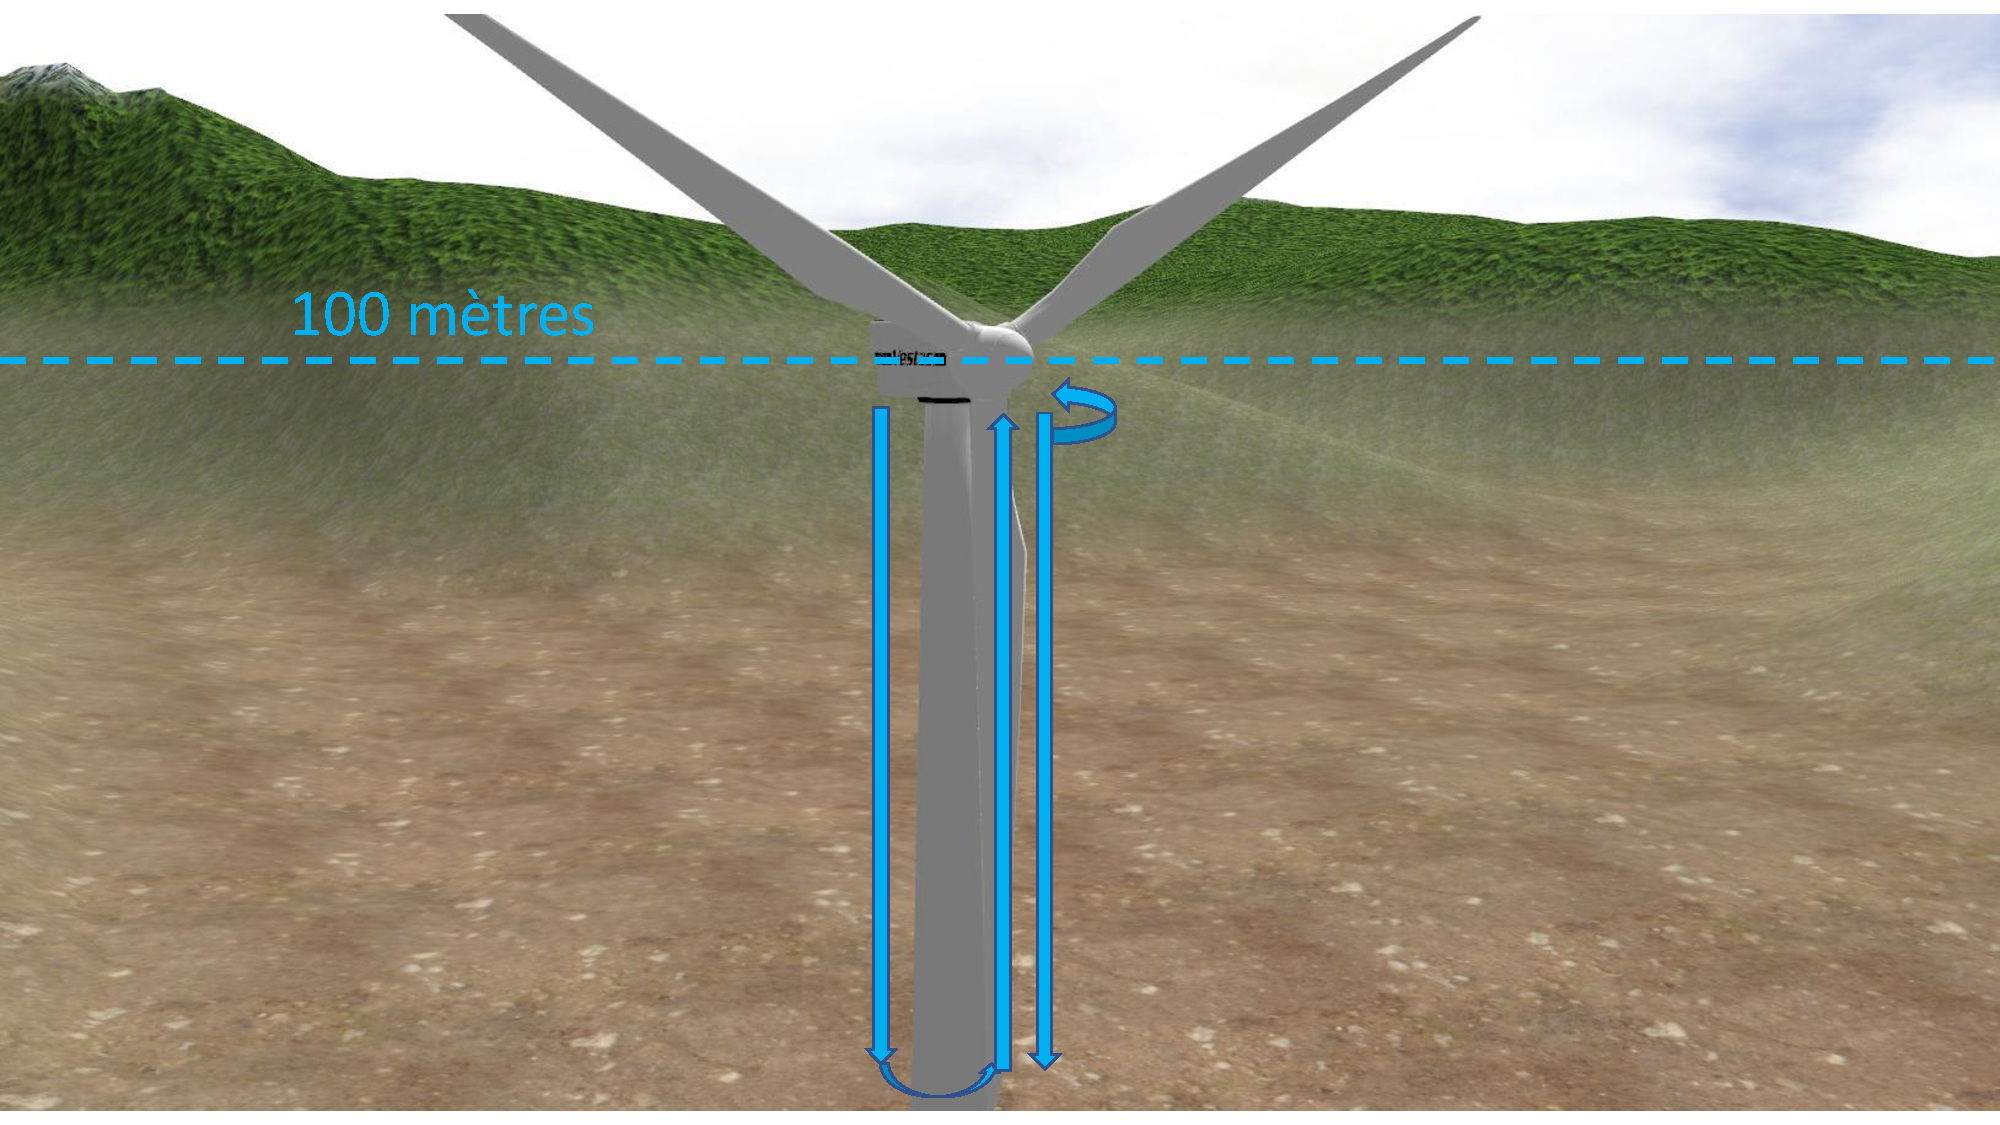
\includegraphics[width=\linewidth]{images/supercoolconcept}
  \caption{Trajectoire alternative pour l'inspection d'une pale à la fois sans besoin de COAS.}
  \label{fig:alternative}
\end{figure}

Pour en revenir à la méthode que nous proposons, l'UAV bénéficierait grandement de l'utilisation de D-GPS ou de GPS-RTK à deux antennes. Le premier avantage serait qu’avec un positionnement plus précis, il serait possible de se rapprocher beaucoup plus de la structure et obtenir de meilleures images. Les distances utilisées en simulation prennent en compte que la précision du positionnement du md4-100 est typiquement entre $\sigma = 1.0$ et $\sigma = 1.5$ mètres. De plus, avec les systèmes à deux receveurs, il n'y aurait plus d'inquiétudes à propos de la zone d'interférence magnétique devant la nacelle.

Bien que ce soit rare, il arrive parfois que la mission échoue lorsque l'UAV perd de vue la pale qu'il est en train de suivre. La cause est habituellement une instabilité lorsque le dernier faisceau du lidar est près de la bordure de la pale. L'UAV tangue pour s'approcher ou reculer et le lidar perd ou regagne la pale. Ce mouvement peut se répéter jusqu'à ce que l'oscillation fasse perdre la pale complètement. Ce problème peut être palié en introduisant une meilleure gestion du cas où le lidar tombe en faute, une procédure de recherche lorsque la pale est perdue et une limite sur l'accélération à la sortie des contrôleurs.

En ce qui concerne les résultats du traitement visuel, il est clair que la méthode proposée ne mérite pas plus d'investigations. Certaines possibilités pourraient être étudiées par exemple après une détection réussie, les descripteurs de caractéristiques tels que \textit{Oriented FAST and Rotated BRIEF} \citep{Rublee2011} pourraient êtres extraits et suivi par un algorithme de flux optique \citep{Lucas1981}. Ceci donnerait une deuxième mesure au filtre de Kalman potentiellement plus fiable. Une autre possibilité serait de remplacer la procédure de détection par un réseau de neurones entièrement convolutionnel qui calculerait conjointement la segmentation et l'orientation des pales. L'une des avenues prometteuses que nous avions commencé à étudier est l'utilisation de filtres non-linéaires tel qu'un filtre à particules pour le suivi et la localisation de l'éolienne \citep{Sugandi2009}. En somme, nous n'écartons pas la possibilité de faire une inspection entièrement par vision, mais ceci devrait être fait au moyen de méthodes plus avancées que celles examinée dans le présent mémoire.

%Nous avions brièvement aussi étudié la possibilité d'utiliser un filtre à particule basé sur la couleur pour le suivi d'une objet basé sur \citep{truong2016object}, par contre puisque
